\section{平面性判定アルゴリズム}
まず深さ優先探索に基づく平面性判定の概要を確認する。
次に子孫のフリンジを継承する際に禁止構造を検出する手順を議論する。
禁止構造を検出しなかった場合のアルゴリズムの正当性についても議論する。


%\paragraph{平面性判定と部分問題としてのフリンジ}
\subsection{平面性判定の概要}%と部分問題としてのフリンジ}

\paragraph{平面性判定の概要のpythonコード}
平面性判定アルゴリズムのフレームワークは
\lstrefname\ref{lst:is_planar}に示すように
橋検出の\lstrefname\ref{lst:dfs_2_edge_connectivity}と本質的には変わらない。
入力として連結なグラフ{\tt G}と任意の頂点{\tt root}が与えられたとき、
{\tt G} の{\tt root}から到達可能な連結成分の平面性を判定する。
ハイライトは橋検出との変更箇所を表している。



%変更箇所は各木辺にクラス{\tt fringe}を対応付ける点である。
%木辺$(x, y)$のフリンジを${\mathcal T}_y$の頂点から$y$の先祖に接続するすべての補木辺とする。
%{\tt fringe}はフリンジ内の各補木辺の終点の高さを管理する。

%\hspace{-1.5em}ある木辺のフリンジのイメージは右図のような感じになる。
%破線の補木辺すべてが木辺$(x,y)$のフリンジに属す。




\begin{lstlisting}[language=Python, caption=is\_planar,escapechar=@,
                   label=lst:is_planar]
def is_planar(G, root):
    stack, dfs_height = [(root, iter(G.neighbors(root)))], {x: -1 for x in G}
    dfs_height[root] = 0
    @\hl{fringes}@ = []
    while stack:
        parent, children = dfs_stack[-1]
        try:
            child = next(children)
            if dfs_heights[child] < 0:
                dfs_height[child] = dfs_height[parent] + 1
                stack.append((y, iter([u for u in G.neighbors(child) if u != parent])))
                @\hl{fringes}@.append([])
            else:
                if dfs_height[parent] > dfs_height[child]:
                    @\hl{fringes[-1].append(fringe(dfs\_height[child]))}@
        except StopIteration:
            stack.pop()
            if len(fringes) > 0:
                @\hl{\mbox{\textcolor{magenta}{try}}:}@
                    @\hl{merge\_fringes(fringes, dfs\_height[stack[-1][0]])}@
                @\hl{\mbox{\textcolor{magenta}{except}} Exception:}@
                    @\hl{\mbox{\textcolor{magenta}{return}} False}@
    return True                   
\end{lstlisting}

第20行目の関数{\tt merge\_fringes}が各木辺のフリンジを形成する手続きで、
禁止グラフを検出したら直ちに例外{\tt Exception}を生成し処理を完了する。
直感的には、
スタックの末尾にいる木辺$(x, y)$のフリンジを形成するために、
%終点$y$に接続している子孫の
$\omega^+(y)$内の各木辺のフリンジを継承し併合することを試みる。



\setcolumnwidth{0.6\textwidth, 0.4\textwidth}
\begin{paracol}{2}
\paragraph{フレームワークの計算量}
フレームワークの計算量が、
条件付きで橋検出と同様に深さ優先探索に準ずる計算量$O(|E|)$となることを確認する。
対象グラフ$G=(V, E)$およびその深さ優先探索木${\mathcal T}=(V, T)$とする。
異なる点は第15・20行目の{\tt fringe}周りの処理である。
第15行はただ一つの補木辺で初期化されるフリンジを生成してスタックに積むだけなので$O(1)$。
全体で$O(|E\setminus T|)$。
第20行はスタックの先頭にある木辺$e=(x, y)$の
$O(|\omega^+(y)|)$個の子孫のフリンジと
$O(|\omega^-(y)|)$個のただ一つの補木辺で構成されるフリンジ
を併合して$\fringe(e)$を形成する。

このとき関数{\tt merge\_fringes}が
$O(|\omega^+(y)|+|\omega^-(y)|)$時間で処理できれば
全体で見ても$O(|E|)$で抑えられる。つまり、\\
$\sum_{(x, y) \in T}O(|\omega^+(y)|+|\omega^-(y)|)=
O(|T|)+O(|E\setminus T|)=O(|E|)$。



\switchcolumn
%\vspace{-0.5em}
\vspace{1.5\intextsep}
\begin{figure}[ht]
\centering
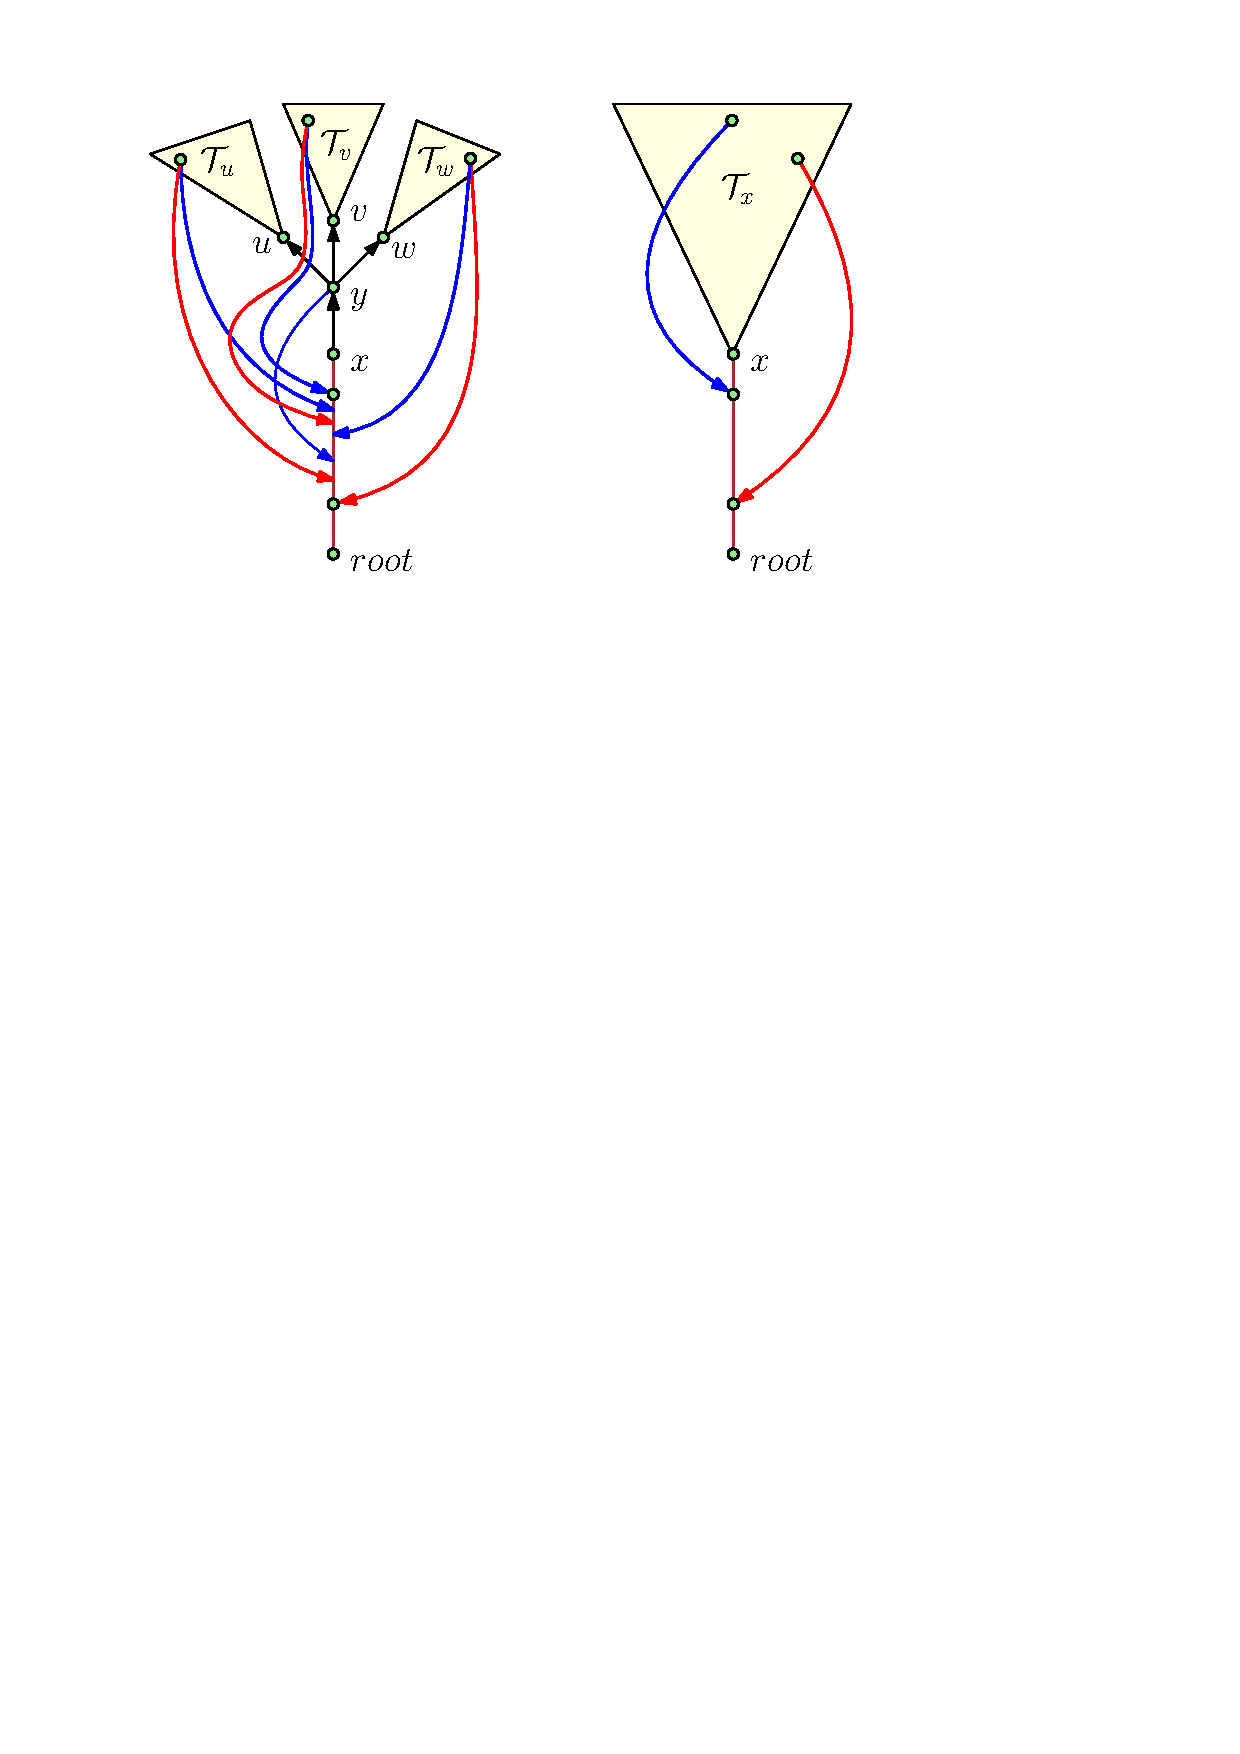
\includegraphics[width=0.39\textwidth]{figures/merging_upper_fringes.pdf}
\end{figure}
\end{paracol}

後述するが、各木辺のフリンジは最も根に近い終点の高さと、
最も根から離れた終点の高さの二つの参照点を備えるだけで十分である。
一つしか補木辺を持たない場合は、それぞれ同じ補木辺を参照する。
二つの子孫間のフリンジの併合は四つの補木辺の終点の高さの比較が主となる。


\setcolumnwidth{0.75\textwidth, 0.25\textwidth}
\begin{paracol}{2}
\paragraph{フリンジの併合と禁止構造}
平面性判定アルゴリズムは、
バックトラックごとにフリンジ内の補木辺が禁止グラフである
クラトフスキーグラフを形成するかを調べる。
%橋検出と同様に禁止グラフを見つけたら、非平面的と判定し処理を完了する。
すべての木辺のフリンジを調べ終わり禁止グラフを検出できなかったら平面的と判定する。

右図は禁止グラフ$K_{3,3}$の細分を含むフリンジの例である。
左は木辺$(x,y)$のフリンジを赤とシアンの矢印の集まりで表している。
各黒辺は木辺とする。右は分かりやすく描画し直した同型のグラフである。
%このようにフリンジは極小な部分問題を定義する重要な役割を果たす。

\switchcolumn
%\begin{figure}[ht]
\vspace{1.\intextsep}
\centering
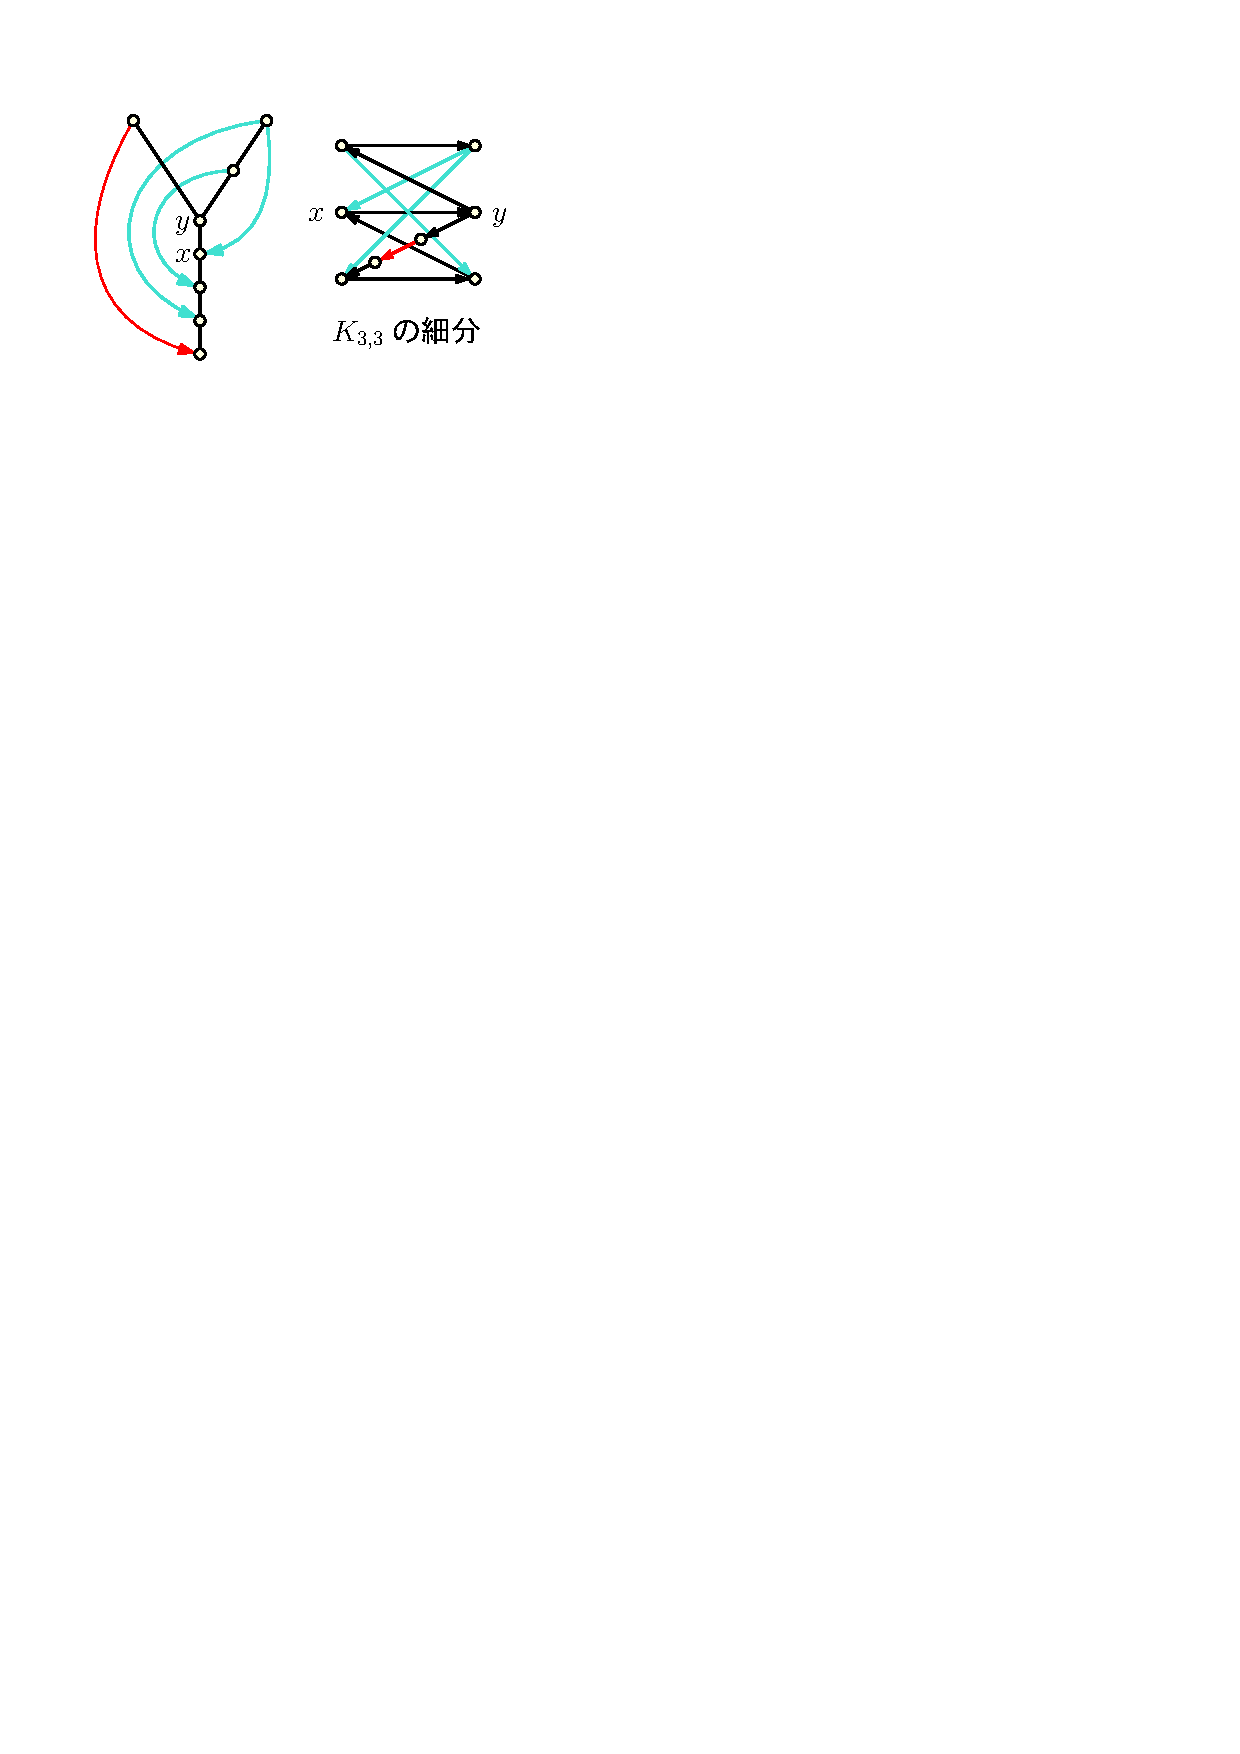
\includegraphics[width=0.24\textwidth]{figures/forbidden_fringe1.pdf}
%\end{figure}
\end{paracol}




\paragraph{継承に基づくフリンジ形成}
%もう少しフリンジの併合の概要が続く。
関数{\tt merge\_fringes}のpythonコードを\lstrefname\ref{lst:merge_fringes}に示す。
関数{\tt get\_merged\_fringes}を用いて
併合したフリンジを取得し(第2行)、
橋検出の場合と同様に不要な補木辺を{\tt fringe}の
クラス関数{\tt prune}を用いて破棄する(第4行)。
%先祖の木辺のフリンジに継承する(第6行)。
第3行の条件式内の{\tt mf is not None}は
$\fringe(e)=\varnothing$で橋の場合の手間を省くための記述である。
第5行の条件式内のクラス変数{\tt fops}は次節で詳説するフリンジ内干渉で
%補木辺の集まりが
極大な非クラフトスキーグラフを見つけるための補木辺の組合せ構造である。
不要な補木辺の破棄で組合せ構造が消滅しない限り先祖のフリンジに継承される(第6行)。

\begin{lstlisting}[language=Python, caption=merge\_fringes,escapechar=@,
                   label=lst:merge_fringes]
def merge_fringes(fringes, dfs_height):
    mf = get_merged_fringe(fringes.pop())
    if mf is not None:
        mf.prune(dfs_height)
        if mf.fops:
            fringes[-1].append(mf)
\end{lstlisting}






\setcolumnwidth{0.66\textwidth, 0.33\textwidth}
\begin{paracol}{2}
\paragraph{フリンジ併合の概要}
\lstrefname\ref{lst:merge_fringes}内で呼ばれる
%関数
{\tt get\_merged\_fringe}は子孫のフリンジリスト
{\tt upper\_fringes}を入力として、
それらを併合したフリンジ{\tt new\_fringe}を出力する。
\lstrefname\ref{lst:get_merged_fringe}はそのpythonコードである。

まず3行目で子孫のフリンジを整列しているが、
各フリンジの最も根に近い補木辺の終点の高さを基準にしている。
右図の例では${\mathcal T}_u < {\mathcal T}_v$となる。
これは根に近い補木辺を持つフリンジほど平面埋込みにおいて
外面に近くあるべきと考えるからである。
第4行以降は、根に近い補木辺を持つものから順に
{\tt fringe}のクラス関数{\tt merge}を用いて併合していく(第5・6行)。

右図は3通りの平面埋込みの例を示しているが、
上段のいずれも最も根に近い補木辺を
持つフリンジの方が外側に来ていることを示している。
下段のように${\mathcal T}_v$の赤線の初等閉路の内側に
${\mathcal T}_u$を埋め込むことはできるが
根も同時に埋め込まなければならず根が外面に現れなくなる。
この状況は後続の処理を複雑にするため好ましくない。
対象グラフが平面的なら
タットのばね\cref{thm:tutte}より
任意の頂点を外面境界上に配置する平面埋込みの存在が保証されるので、
深さ優先探索の根は外面に属す平面埋込みに制限する。
従って下段の平面埋込みは拒否される。



\switchcolumn
%\vspace{-0.5em}
\vspace{1.5\intextsep}
%\begin{figure}[ht]
\centering
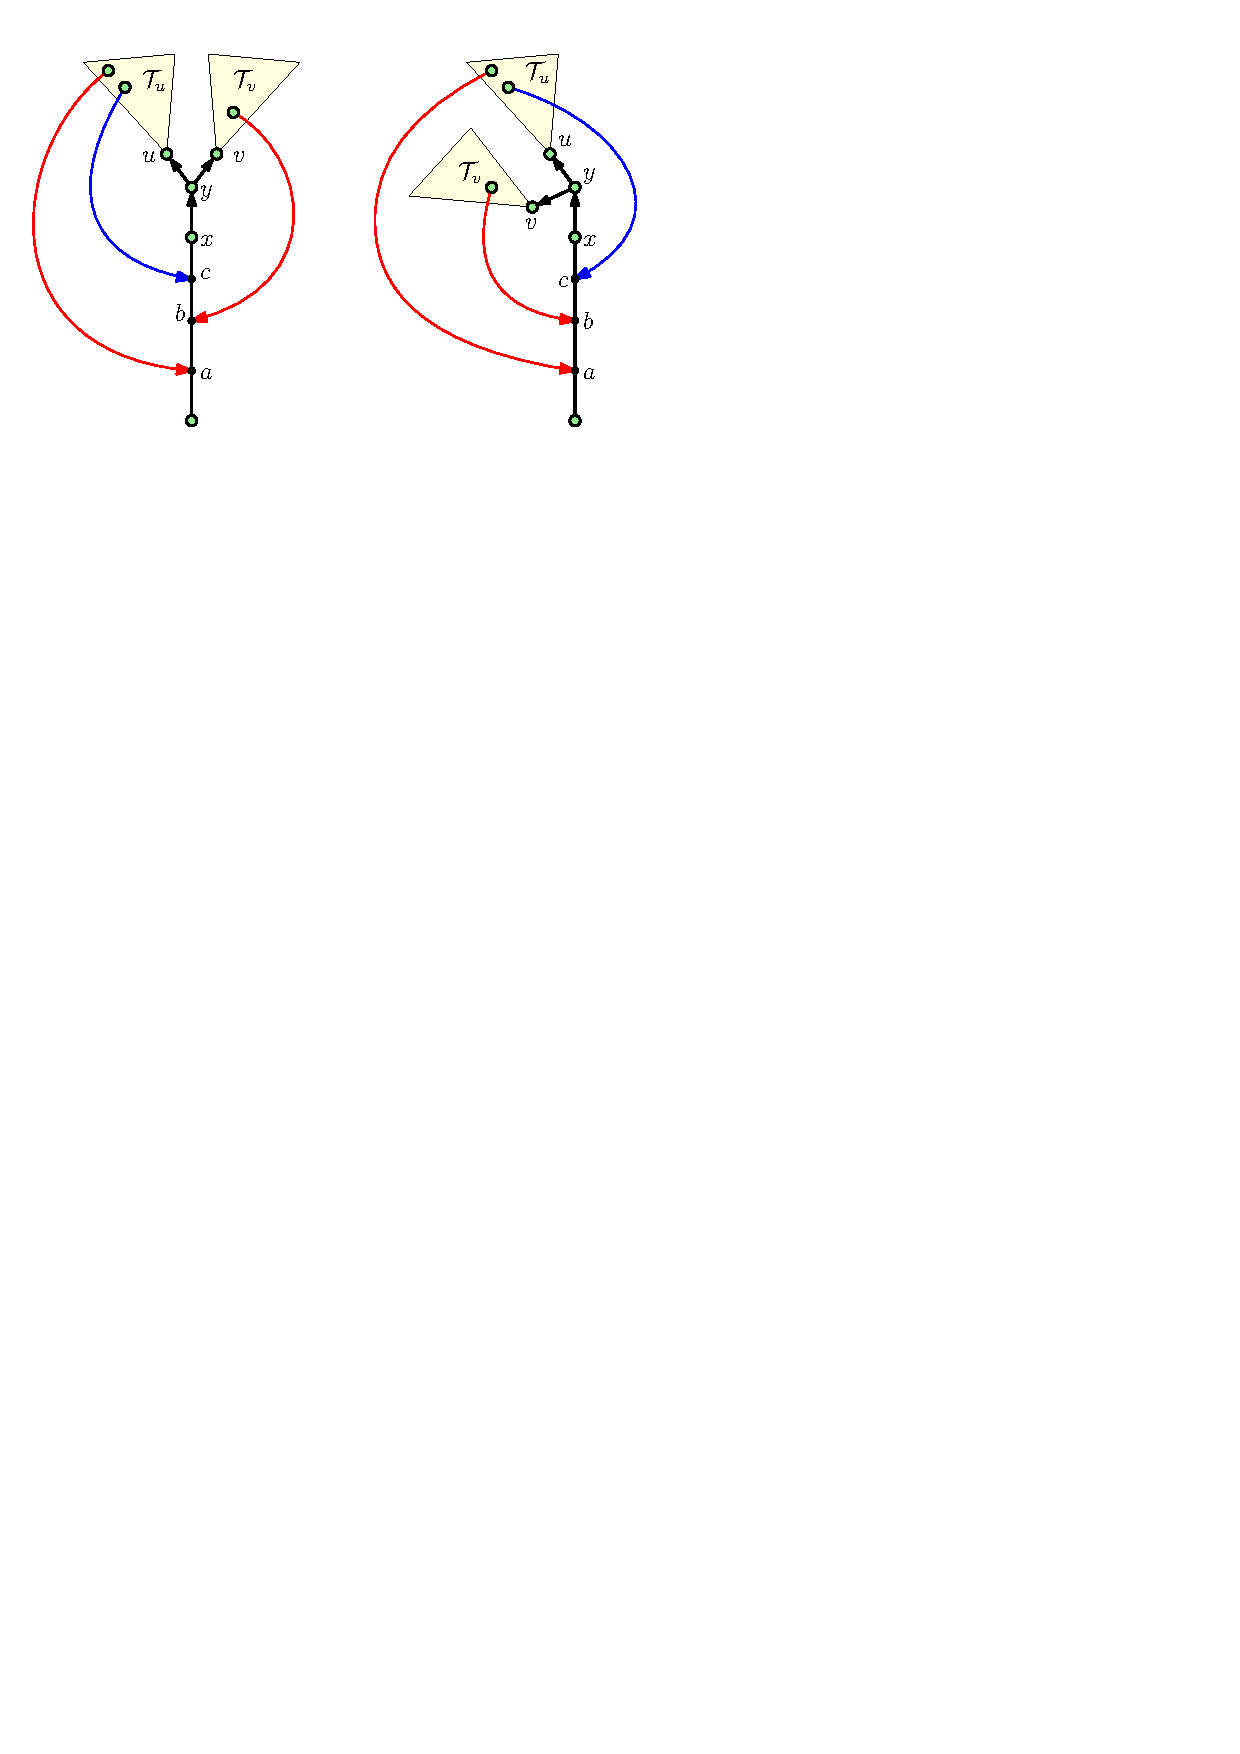
\includegraphics[width=0.32\textwidth]{figures/get_merged_fringe.pdf}\\
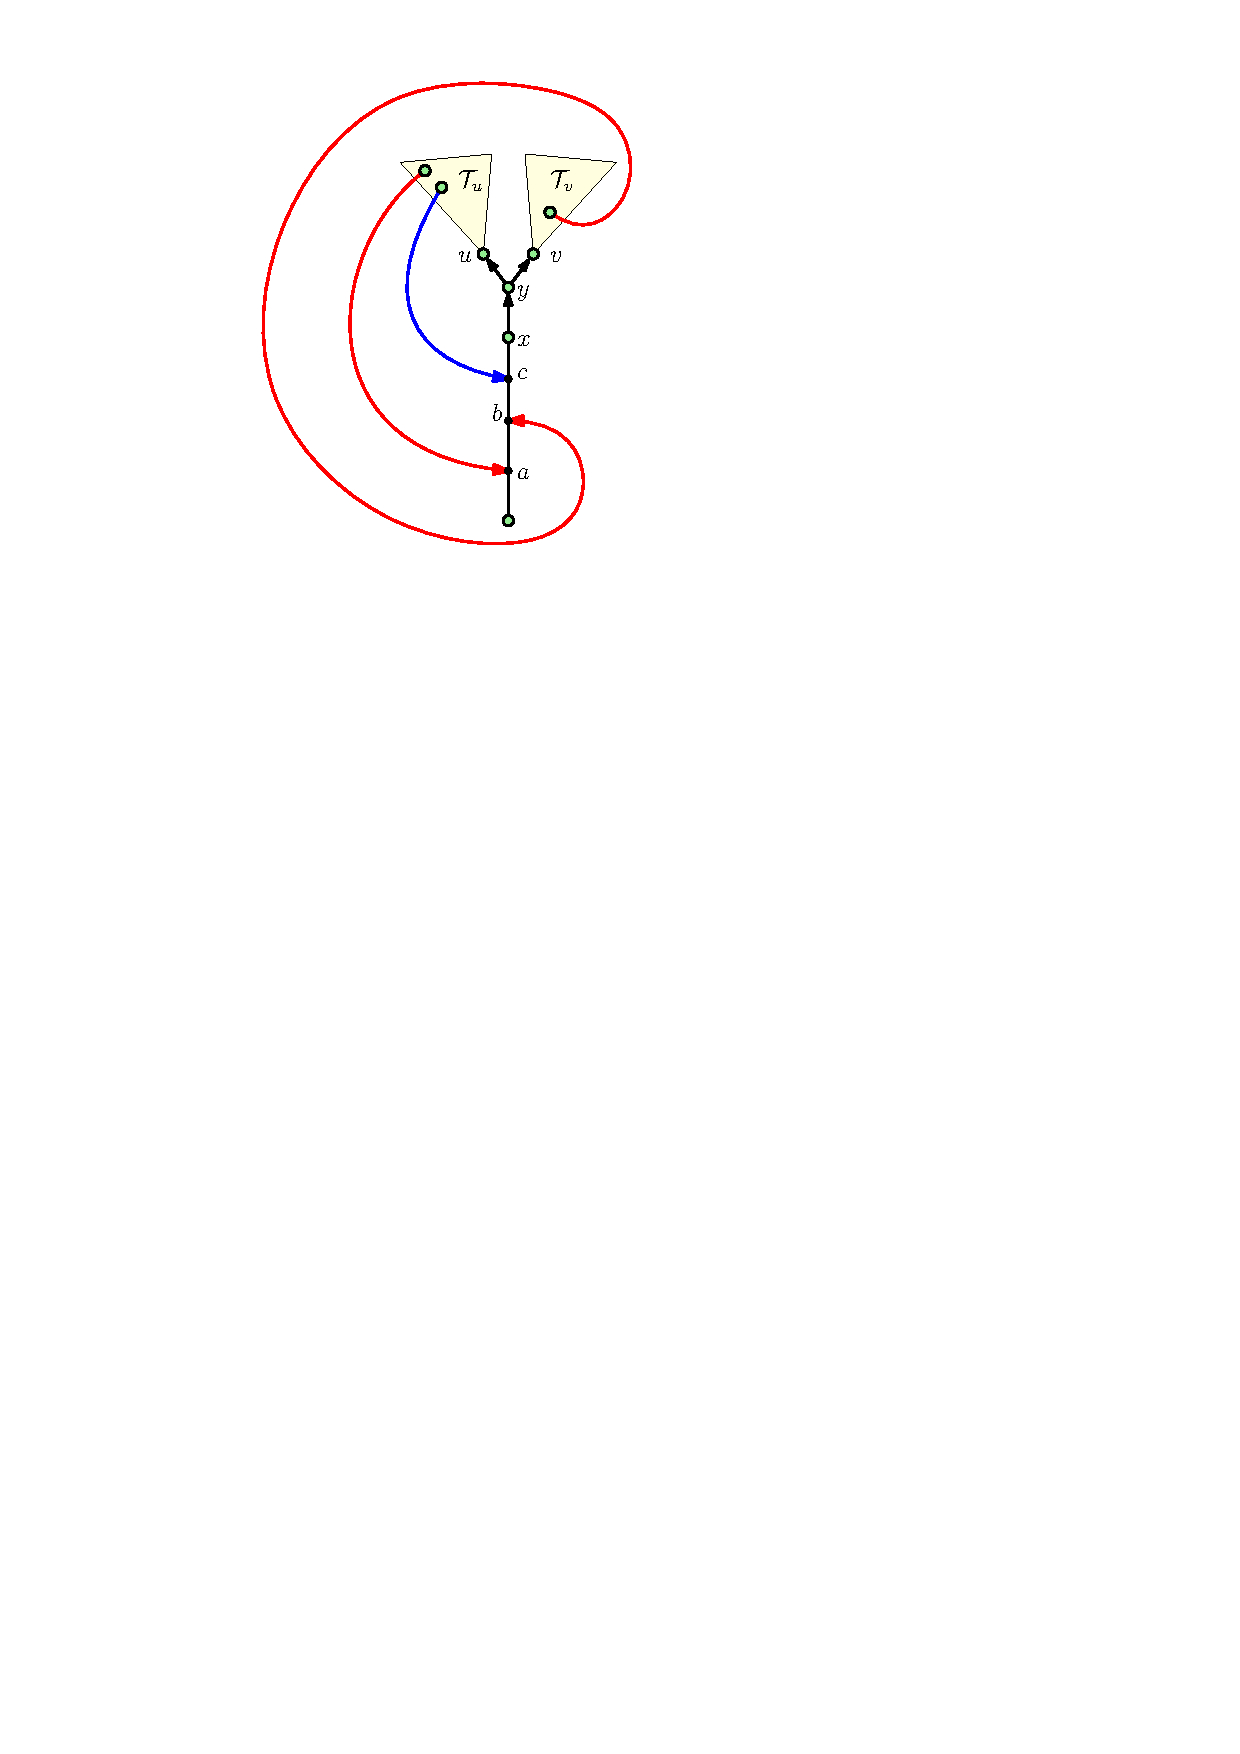
\includegraphics[width=0.16\textwidth]{figures/get_merged_fringe2.pdf}
%\end{figure}
\end{paracol}



\begin{lstlisting}[language=Python, caption=get\_merged\_fringe,escapechar=@,
                   label=lst:get_merged_fringe]
def get_merged_fringe(upper_fringes):
    if len(upper_fringes) > 0:
        upper_fringes.sort()
        new_fringe = upper_fringes[0]
        for f in islice(upper_fringes, 1, len(upper_fringes)):
            new_fringe.merge(f)
        return new_fringe
\end{lstlisting}

\paragraph{整列アルゴリズムについて}
\lstrefname\ref{lst:get_merged_fringe}は
整列アルゴリズムとしてpythonバインドのTimSortを用いているが、
厳密には整数整列アルゴリズムで実装しなければならない。
補木辺の終点の高さは整数なのでビンソートなどを用いれば、
$O(|\omega^+(v)|+|\omega^-(v)|)$時間で処理できる。
各頂点$v$の$\omega^+(v)$および$\omega^-(v)$のサイズの分布を見て
必要に応じて適した整数ソートを実装すると良い。





%%%%%%%%%%%%%%%%%%%%%%%%%%%%%%%%%%%%%%%%%%%%%%%%%%%%%%%%%%%%%%%%%%%%%%%%%%%%%%%%%
\subsection{フリンジの基本的な性質}

フリンジは対象の木辺に関連づく補木辺の集まりであるが、
リストで管理するには簡潔すぎる。
禁止グラフを形成しそうな補木辺の集まりを構造化し、
これをリストする。
禁止グラフを形成しそうな組合せ構造をフリンジ内干渉と呼ぶ。

\subsubsection{フリンジの基本構造}

下記にフリンジクラスのpythonコードの一部を示す。
クラスメソッドなど詳細を含めたコードは節末の\lstrefname\ref{fringe}に示す。
初期化は、空集合もしくは一つの補木辺からなる集合の二通りを受け付け、
クラス{\tt fop}の双方向キュー{\tt self.fops}を作る。

\vspace{-1.\intextsep}
\setcolumnwidth{0.85\textwidth, 0.15\textwidth}
\begin{paracol}{2}
%\begin{lstlisting}[language=Python, caption=クラス fringe,
\begin{lstlisting}[language=Python]
class fringe:
    def __init__(self, dfs_h=None):
        self.fops = deque() if dfs_h is None else deque([fop(dfs_h)])

    @property
    def H(self):
        return self.fops[0]

    @property
    def L(self):
        return self.fops[-1]
\end{lstlisting}

\switchcolumn
\vspace*{2.\intextsep}
\centering
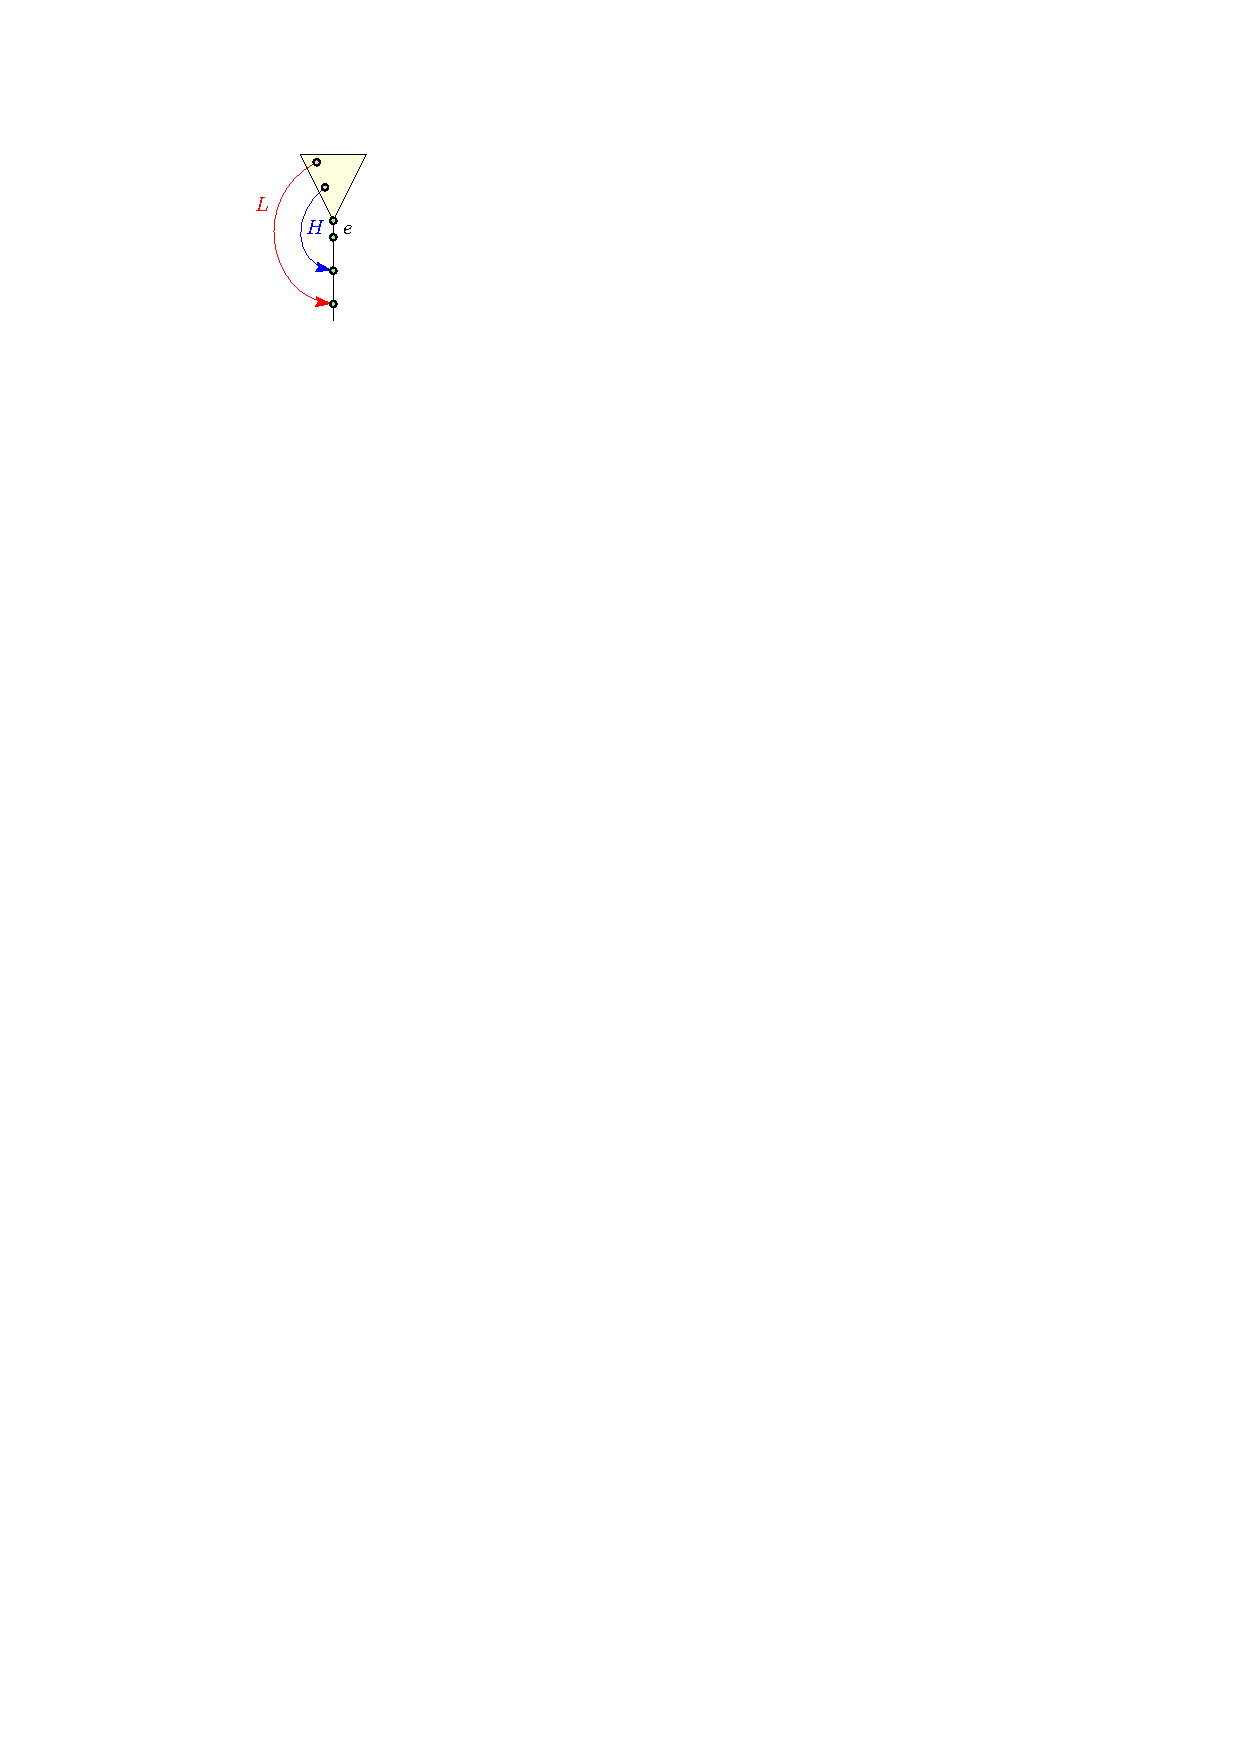
\includegraphics[width=0.11\textwidth]{figures/fringe_basic_code.pdf}
\end{paracol}

フリンジの基本構造は、二つの参照点{\tt L, H}しか持たない簡潔な構造をとる。
{\tt L, H}それぞれ最も根に近い、もしくは遠い終点を持つ補木辺への参照を与える。
フリンジ内のフリンジ内干渉のリストを加工する際、
内側から、すなわち{\tt H}から更新や削除がされる。
{\tt L}はフリンジ内干渉を形成する補木辺の判定で用いられる。







\subsubsection{フリンジ内干渉の定義}

\setcolumnwidth{0.66\textwidth, 0.33\textwidth}
\begin{paracol}{2}
\begin{definition}[フリンジ内干渉]
$v \in V$および$e_1, e_2 \in \omega^+(v)$とする。
$e_1$が橋でないなら、
$e_2$の$e_1$に対するフリンジ内干渉を次のように定義する。
\[
\fop_{e_1}(e_2)=\{(x, y) \in \fringe(e_2) ~:~ y \succ \low(e_1)\}.
\]
$e_1$が橋なら$\fop_{e_1}(e_2) = \varnothing$とする。

また、木辺$e=(x, y)$と補木辺$f=(y, y') \in \omega^-(y)$に対する
フリンジ内干渉も同様に定義する。
$e$が橋でないなら、
\begin{align*}
\fop_e(f) &= \{f ~:~ y' \succ \low(e)\},\\
\fop_f(e) &= \{(x, y) \in \fringe(e) ~:~ y \succ y'\}.
\end{align*}
$e$が橋なら$\fop_e(f)=\varnothing$とする。
\end{definition}




\switchcolumn
\vspace{-1.5\intextsep}
\centering
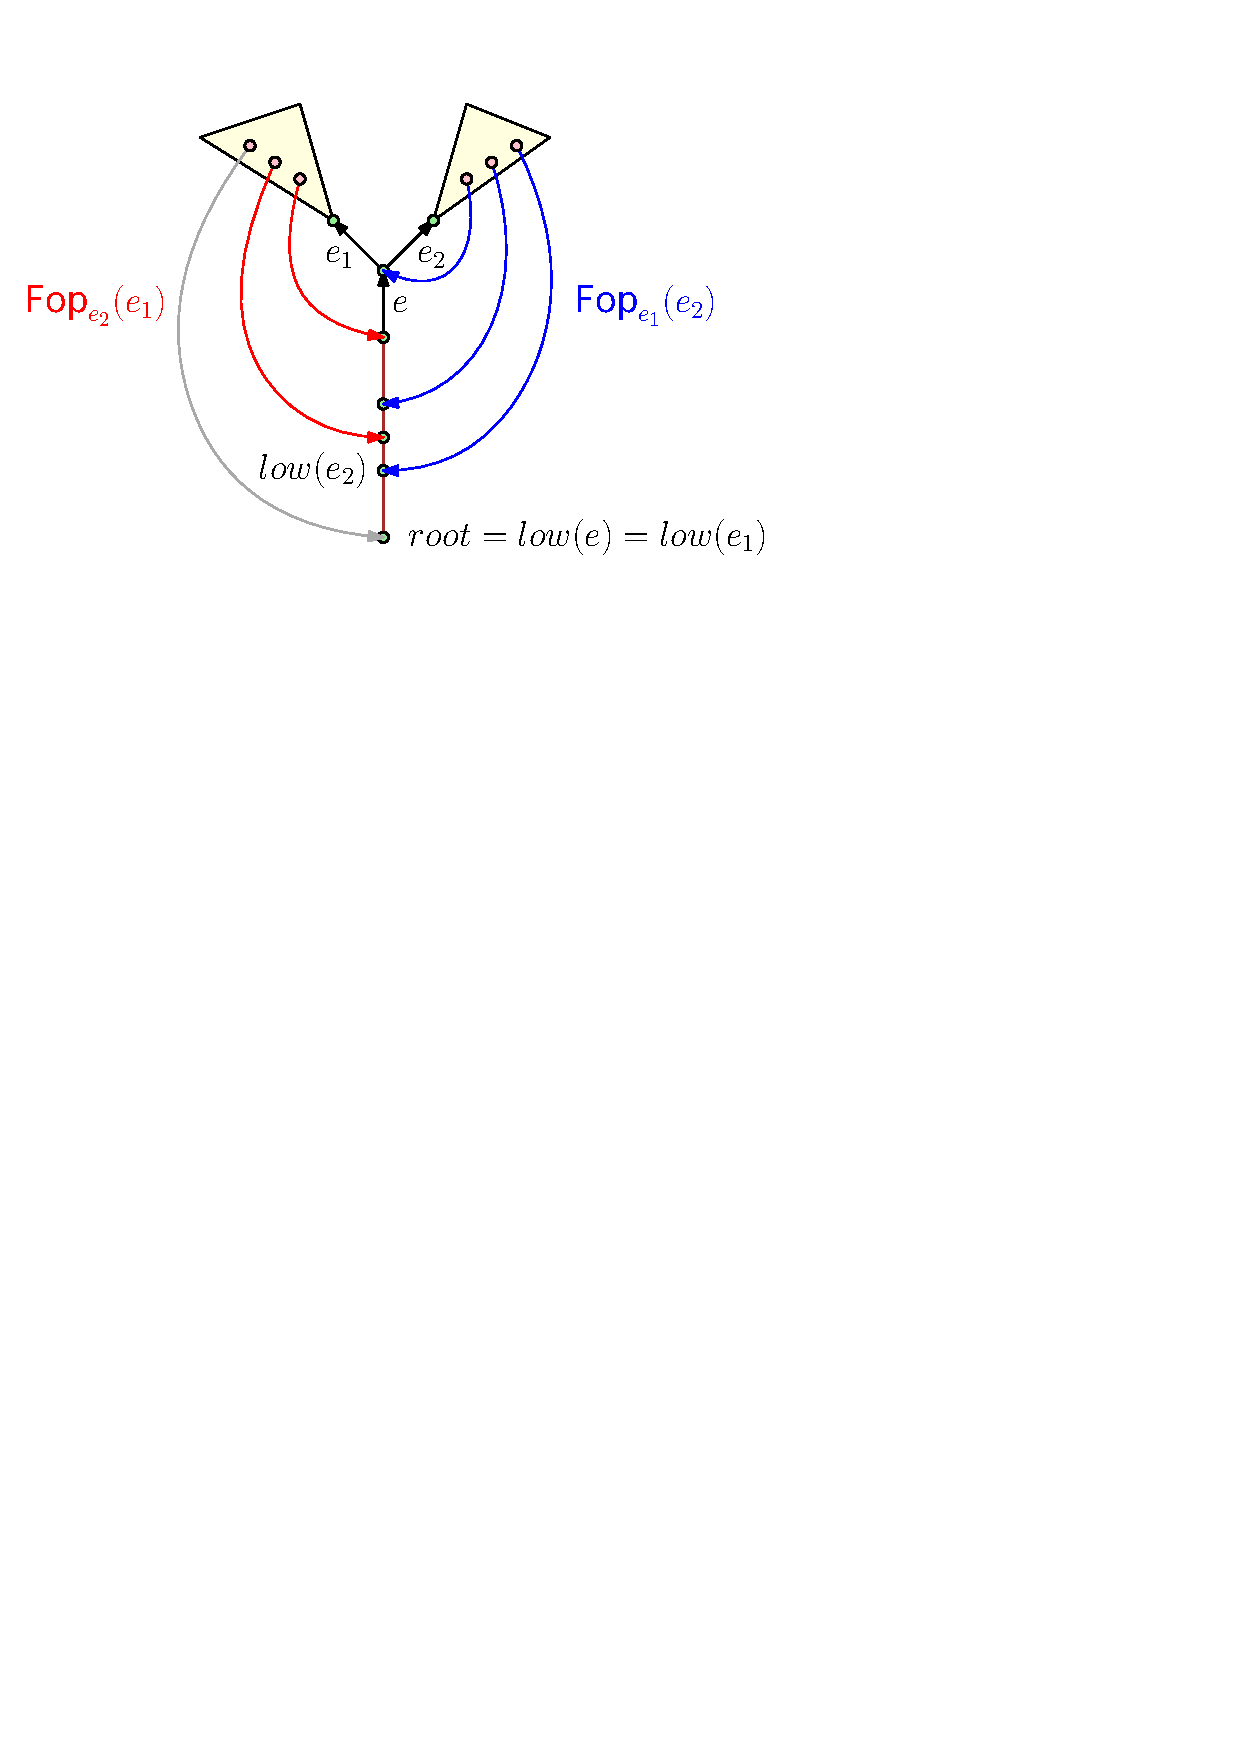
\includegraphics[width=0.3\textwidth]{figures/fop_and_low_1.pdf}

\vspace{0.5\intextsep}
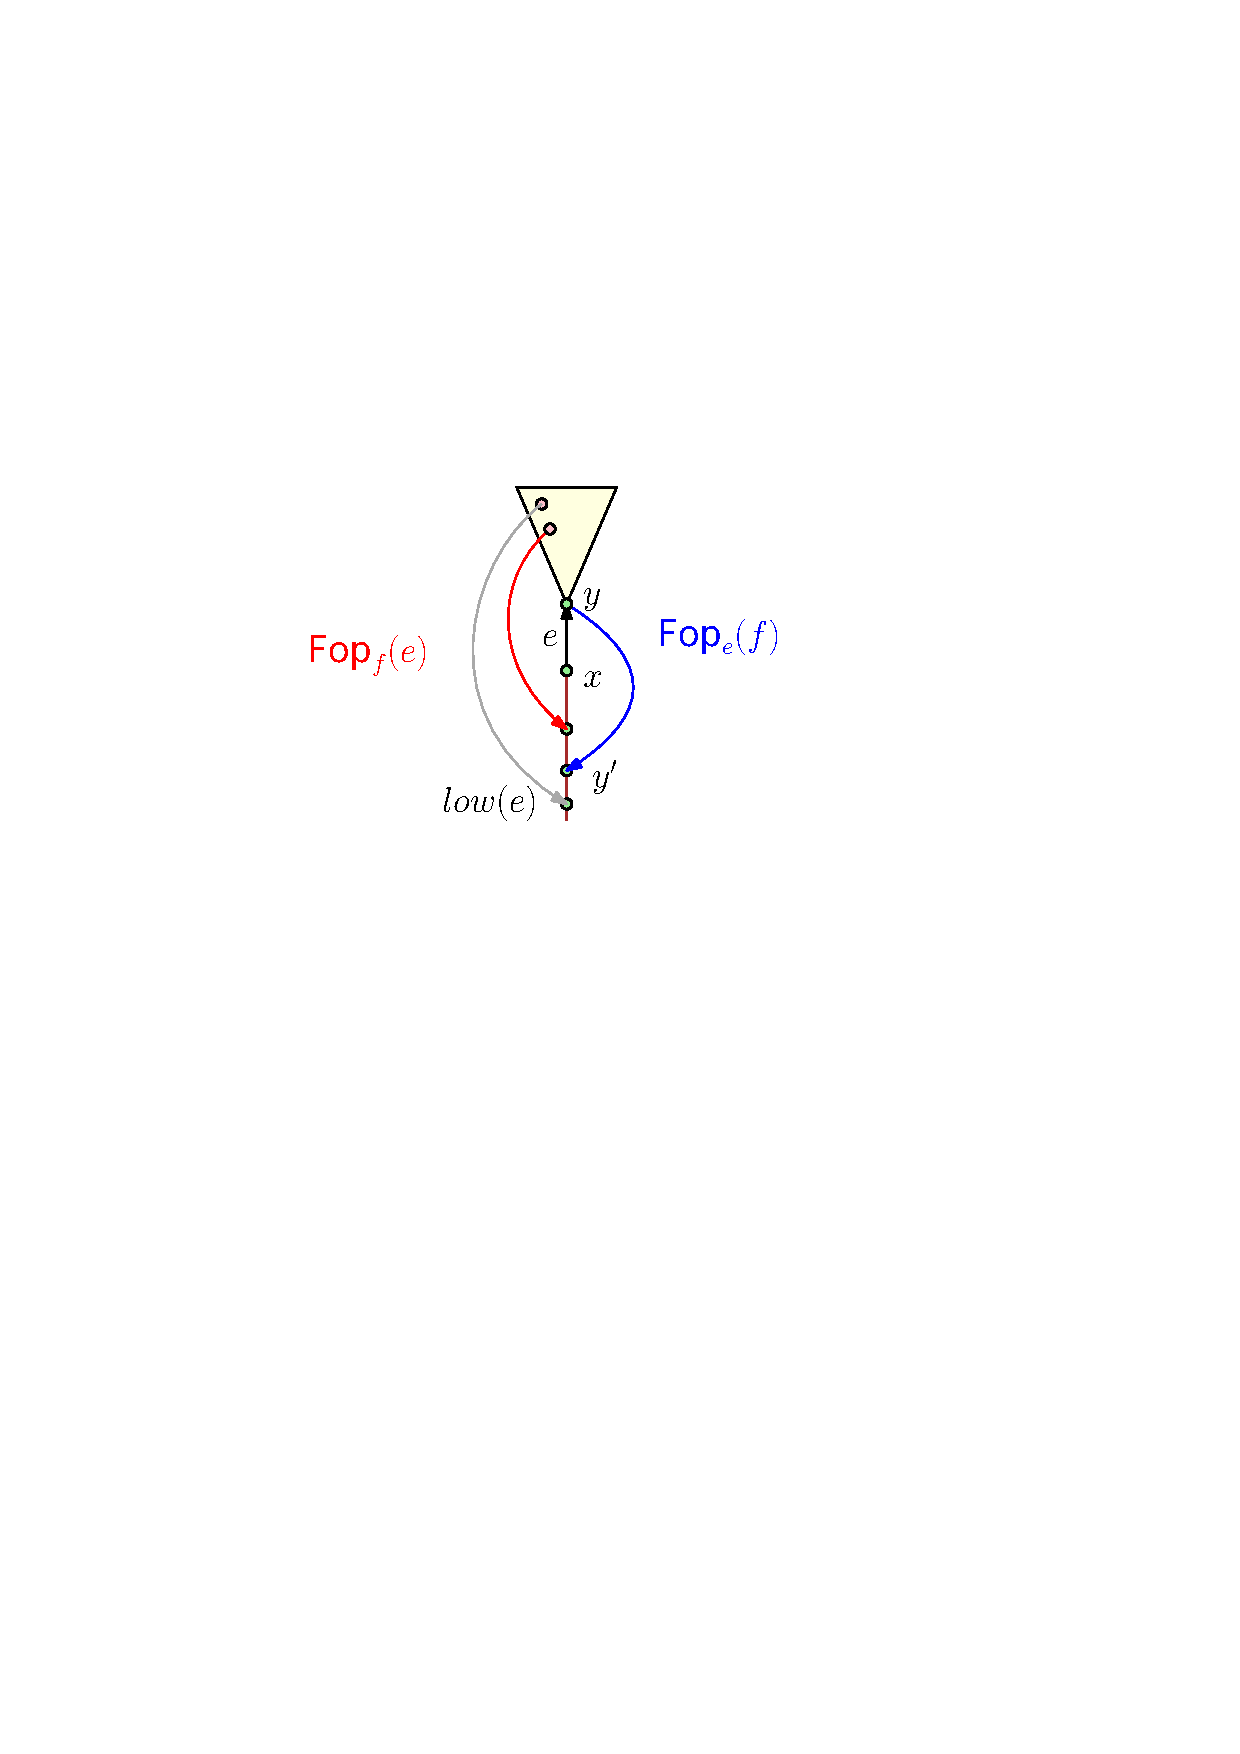
\includegraphics[width=0.22\textwidth]{figures/fop_and_low_2.pdf}
\end{paracol}





\begin{definition}
深さ優先探索木${\mathcal T}=(V, T)$において、
辺集合$T$から頂点集合$V$への写像$\low$を次のように定義する。
\[
\low(e)=\left\{
\begin{array}{ll}
    \argmin_{v\in\tau(e)}\, h(v) ~~~~~~~~ & {\rm if}\ e\ {\rm is\ not\ a\ bridge,} \\
    \bot ~~~~~~~~~~~ & {\rm otherwise.}
\end{array}\right.
\]
ただし、$\tau(e)=\{y ~{\rm for}~ (x, y) \in \fringe(e)\}$とする。
\end{definition}




$\fop_{e_1}(e_2)$と$\fop_{e_2}(e_1)$に属す辺どうし、および
$\fop_e(f)$と$\fop_f(e)$に属す辺どうしは互いに干渉するという。







\subsubsection{フリンジ内干渉のデータ構造}
フリンジ内干渉のデータ構造を\lstrefname\ref{lst:fringe_opposed_subset}に示す。
二つの双方向キューからなる単純な構造だが、
使い方に注意が必要である。
配列{\tt self.c}の二つの双方向キューは、
対象の木辺$(x, y)$に対して${\mathcal T}_y$内の頂点を始点に持ち、
$y$の先祖に終点を持つ%木辺$e_1, e_2$の
互いに干渉する補木辺を管理する。


\setcolumnwidth{0.6\textwidth, 0.4\textwidth}
\begin{paracol}{2}
%\vspace*{-2.\intextsep}
\begin{lstlisting}[language=Python, caption=fringe\_opposed\_subset,escapechar=!,
                   label=lst:fringe_opposed_subset]
class fop:
    def __init__(self, h):
        self.c = [deque([h]), deque()]

    @property
    def left(self):
        return self.c[0]

    @property
    def right(self):
        return self.c[1]

    @property
    def l_lo(self):
        return self.c[0][-1]

    @property
    def l_hi(self):
        return self.c[0][0]

    @property
    def r_lo(self):
        return self.c[1][-1]

    @property
    def r_hi(self):
        return self.c[1][0]
\end{lstlisting}

\switchcolumn
\vspace*{.5\intextsep}

\paragraph{6つの参照点}
ある平面埋込みの木辺$e$のフリンジ内干渉を管理する
データ構造の簡略図を下に示している。
データ構造は6つの参照点を持つ。
左右の双方向キューへの参照{\tt left, right}、
およびそれらの先頭{\tt l\_hi, r\_hi}と末尾{\tt l\_lo, r\_lo}への参照。

\vspace{0.5\intextsep}
%\centering
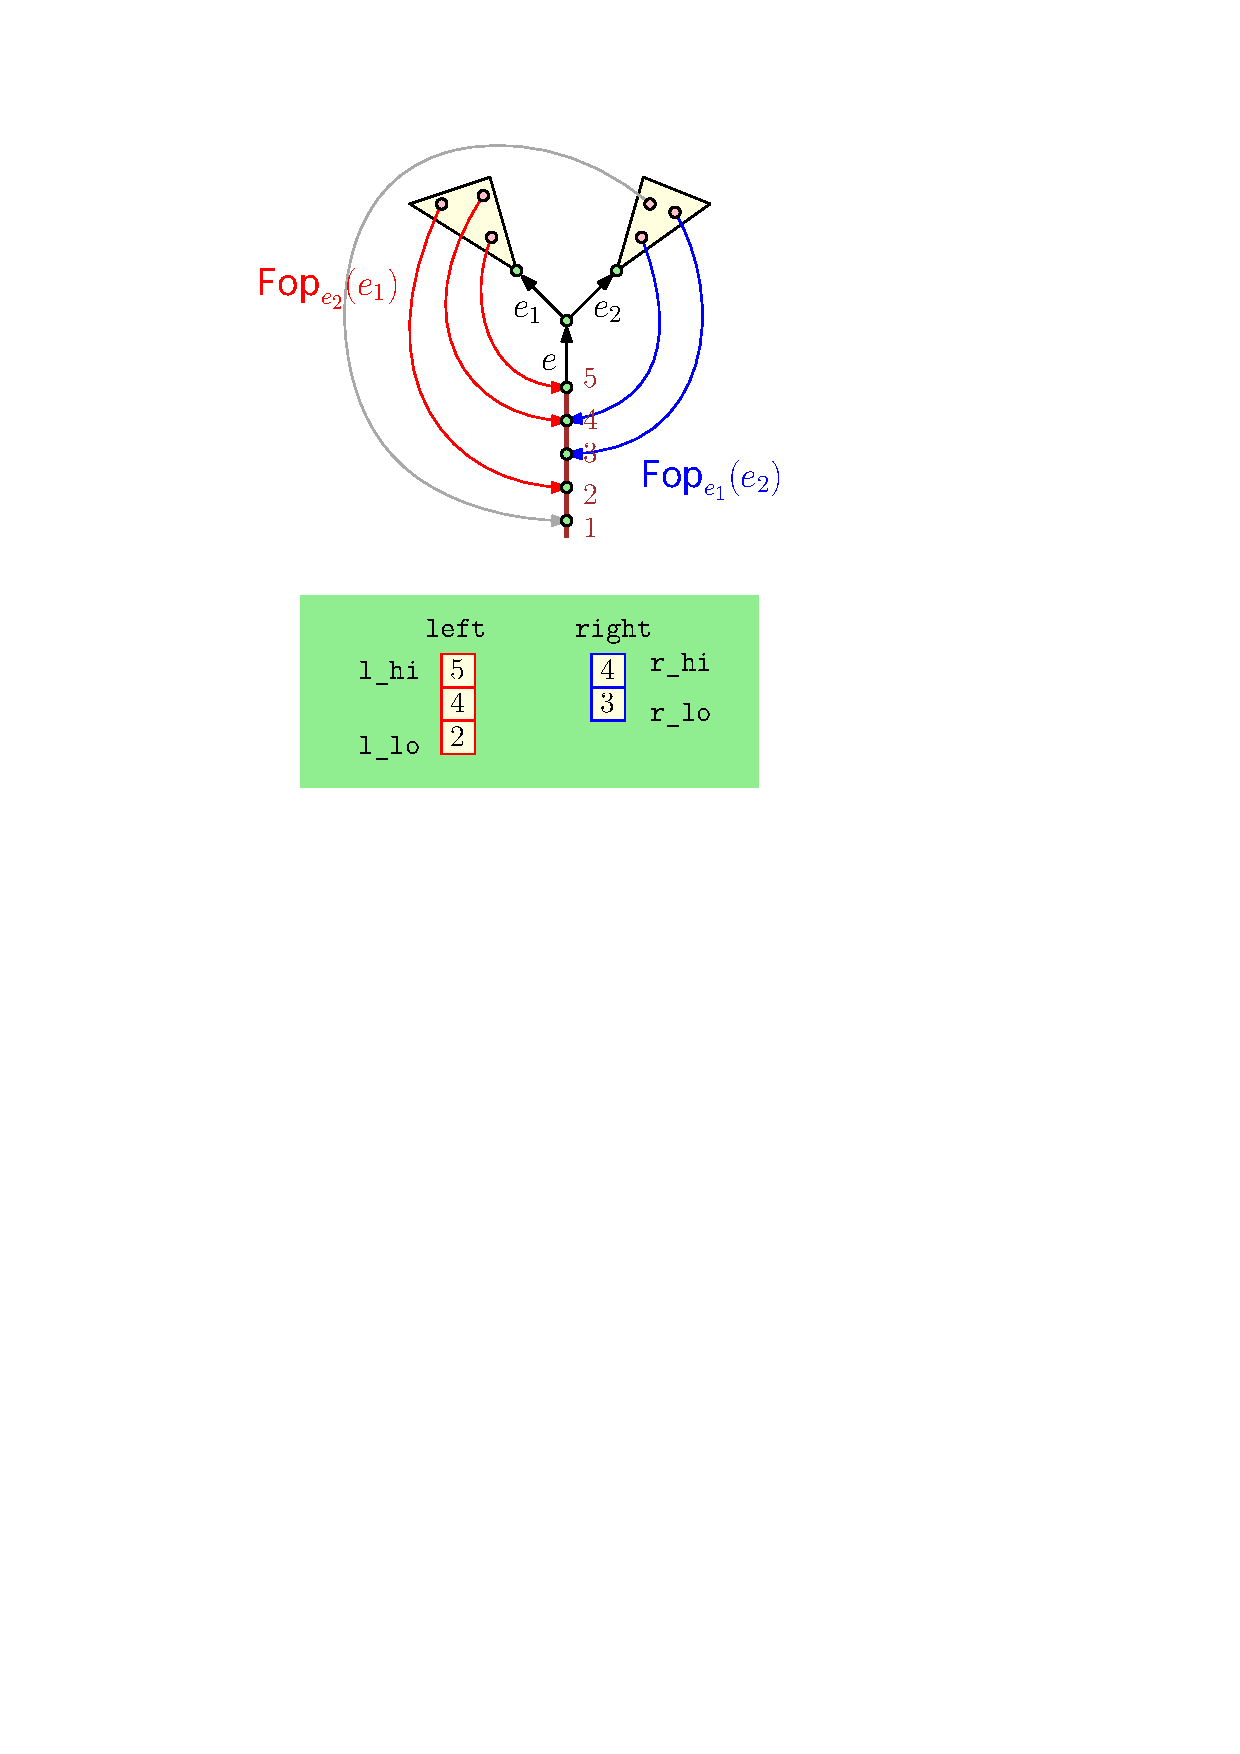
\includegraphics[width=0.27\textwidth]{figures/ds_of_fops.pdf}


\end{paracol}


%%%%%%%%%%%%%%%%%%%%%%%%%%%%%%%%%%%%%%%%%%%%%%%%%%%%%%%%%%%%%%%%%%%%%%%%%%%%%
%\begin{comment}
\paragraph{フリンジ内干渉の文字列表現}
フリンジ内干渉を各補木辺の終点の高さを管理する二つの整数系列の対で表現する。
%この整数は各補木辺の終点の高さを表す。
上図の緑の矩形に囲まれたフリンジ内干渉のデータ構造は%表現 $\varphi$ は
$\varphi=([5,4,2], [4,3])$ のように書ける。
$\varphi$.left.lowで% とアクセスすることで
$\low(e_1)$の高さ$2$を得る。%を取得できる。
%また、上図の灰色の補木辺は別のフリンジ内干渉で定義され$([1], [~])$のように書ける。
%\end{comment}
%%%%%%%%%%%%%%%%%%%%%%%%%%%%%%%%%%%%%%%%%%%%%%%%%%%%%%%%%%%%%%%%%%%%%%%%%%%


\subsubsection{フリンジ内干渉のデータ構造に対する管理規約}
\label{fop_specification}
\paragraph{左優先の管理規約}
各補木辺は可能な限り左側の双方向キューで管理する。
右側の双方向キューは空集合であることが望ましい。
%右が非空である場合は$\varphi$.left.low $< \varphi$.right.low 
%となるようにする。
アルゴリズムの処理過程で左が空集合で右が非空となる場合がある。
その場合、右側の補木辺集合を左に置き換える。
置き換えても問題無いことは\cref{lemma:swap_side}が保証する。


%%%%%%%%%%%%%%%%%%%%%%%%%%%%%%%%%%%%%%%%%%%%%%%%%%%%%%%%%%%%%%%%%%%%%%%
\begin{comment}
\begin{lemma}
フリンジ内干渉の{\tt left}が空で{\tt right}が非空の場合、
{\tt right}の補木辺を{\tt left}に移動させても部分的な平面性は破綻しない。
\end{lemma}

\begin{proof}

\end{proof}
\end{comment}
%%%%%%%%%%%%%%%%%%%%%%%%%%%%%%%%%%%%%%%%%%%%%%%%%%%%%%%%%%%%%%%%%%%%%





\paragraph{補木辺の位相不変性}
平面性判定の処理過程において、フリンジ併合および補木辺除去によって
各双方向キュー内の終点の高さに関する非増加順序を乱さないことを保証しなければならない。
この不変性により、補木辺どうしの干渉性、
あるフリンジを別のフリンジの入れ子にできるかどうか、
不要になった補木辺の除去などの手続きが
定数時間で処理できることを保証できる。
このフリンジ内干渉の位相不変性は、
アルゴリズムの線形時間計算量を保証する上で最重要事項である。






\paragraph{フリンジ内干渉の取り扱い}
管理規約に従うと干渉し合う補木辺の入れ替えは、
具体的に\lstrefname\ref{lst:t_opposite}のように
{\tt fringe}のクラスメソッド{\tt \_merge\_t\_opposite\_edges\_into}として記述できる。
双方向キュー{\tt left}は{\tt right}の末尾に連結されるので$O(1)$時間で完了する。
従って計算量は、
第2行のループ回数$O(|\omega^+(v)| + |\omega^-(v)|)$で抑えられる。


%{\tt left}の補木辺は一度{\tt right}に
%移されたら戻ることはないので$O(|\omega^+(v)|+|\omega^-(v)|)$時間で完了する。
\setcolumnwidth{0.75\textwidth, 0.25\textwidth}
\begin{paracol}{2}
%\vspace{-2.\intextsep}
\begin{lstlisting}[language=Python, caption=\_merge\_t\_opposite\_edges\_into,
                   label=lst:t_opposite]
    def _merge_t_opposite_edges_into(self, other):
        while (not self.H.right and self.H.l_hi > other.H.l_lo):
            other.H.right.extend(self.H.left)
            self.fops.popleft()
\end{lstlisting}

\switchcolumn
\vspace{0.5\intextsep}
\centering
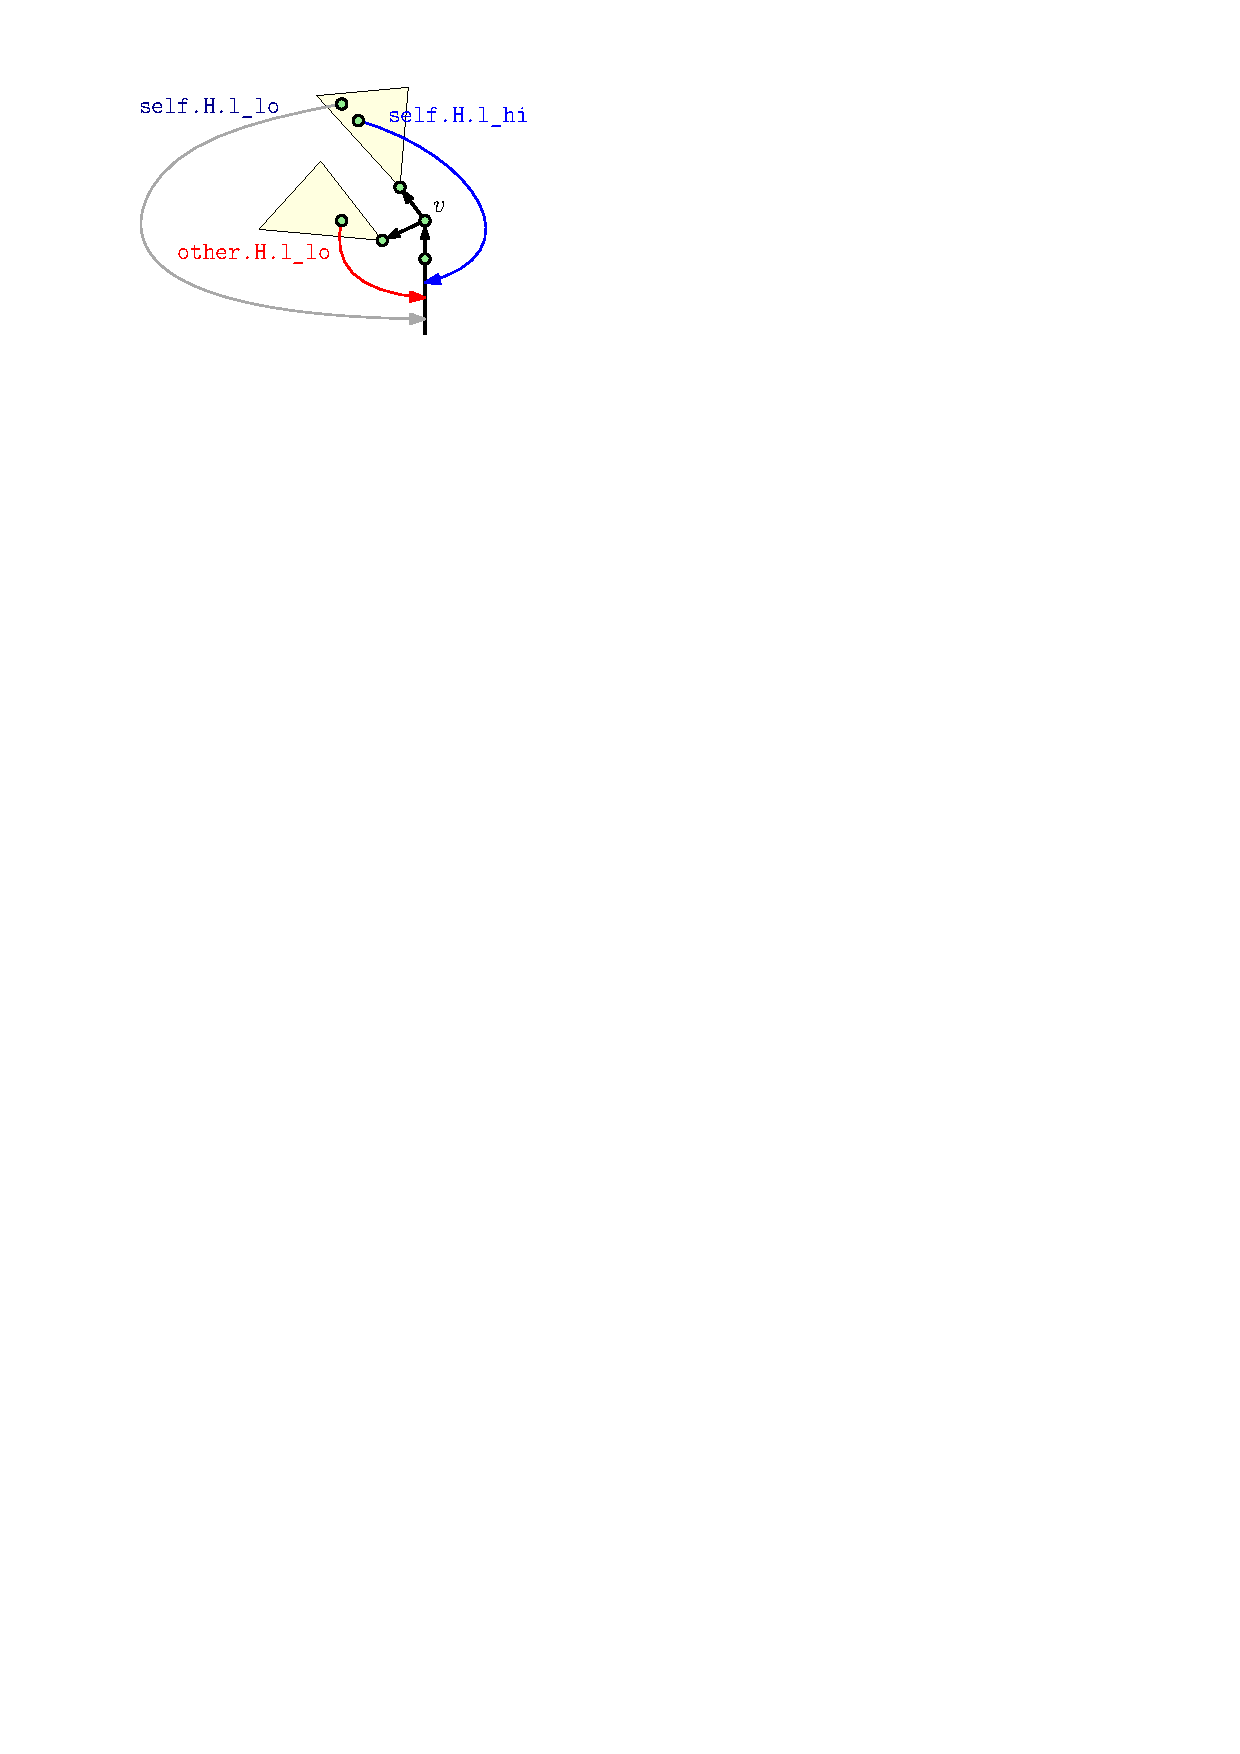
\includegraphics[width=0.24\textwidth]{figures/t_opposite.pdf}
\end{paracol}












%%%%%%%%%%%%%%%%%%%%%%%%%%%%%%%%%%%%%%%%%%%%%%%%%%%%%%%%%%%%%%%%%%%%%%%%%%%%%%%%%%%%%%%%%
\subsubsection{フリンジ内干渉を利用したクラトフスキー部分グラフの検出}

フリンジ内干渉の{\tt right}が非空の場合、その初等閉路の集まりが誘導する部分グラフが
極大な非クラストフキーグラフを形成することを確認する。
つまり
{\tt right}が非空の状態で内から外へ接続する補木辺が存在するとき、
直ちに非平面的と判定できることを示す。
%ここでは、具体的な検出手続きを記述し、その計算量と正当性を考察する。





\setcolumnwidth{0.66\textwidth, 0.33\textwidth}
\begin{paracol}{2}
\paragraph{子孫フリンジの縮約}
最初の例は、
フリンジ内干渉の{\tt left}サイドに補木辺の集まりを仮想的に縮約する手続きである。
具体的な pythonコードを\lstrefname\ref{lst:_merge_t_alike_edges}に示す。
まずは状況確認から。
木辺$e=(x,y)$のフリンジ$\fringe(e)$を形成しようとしている。
このとき子孫の木辺$e_i \in \omega^+(y)$の各フリンジは形成済みであり、
それぞれクラトフスキーグラフを含まない、つまり平面的とする。
また、$k=|\omega^+(y)|$とし、
$e_1, \ldots, e_k$は$h(\low(e_i))$に関して昇順に採番されている。
縮約対象は各木辺$e_2, \ldots, e_k$の各フリンジ内干渉のリスト{\tt fops}である。


\switchcolumn
\vspace{.5\intextsep}
\centering
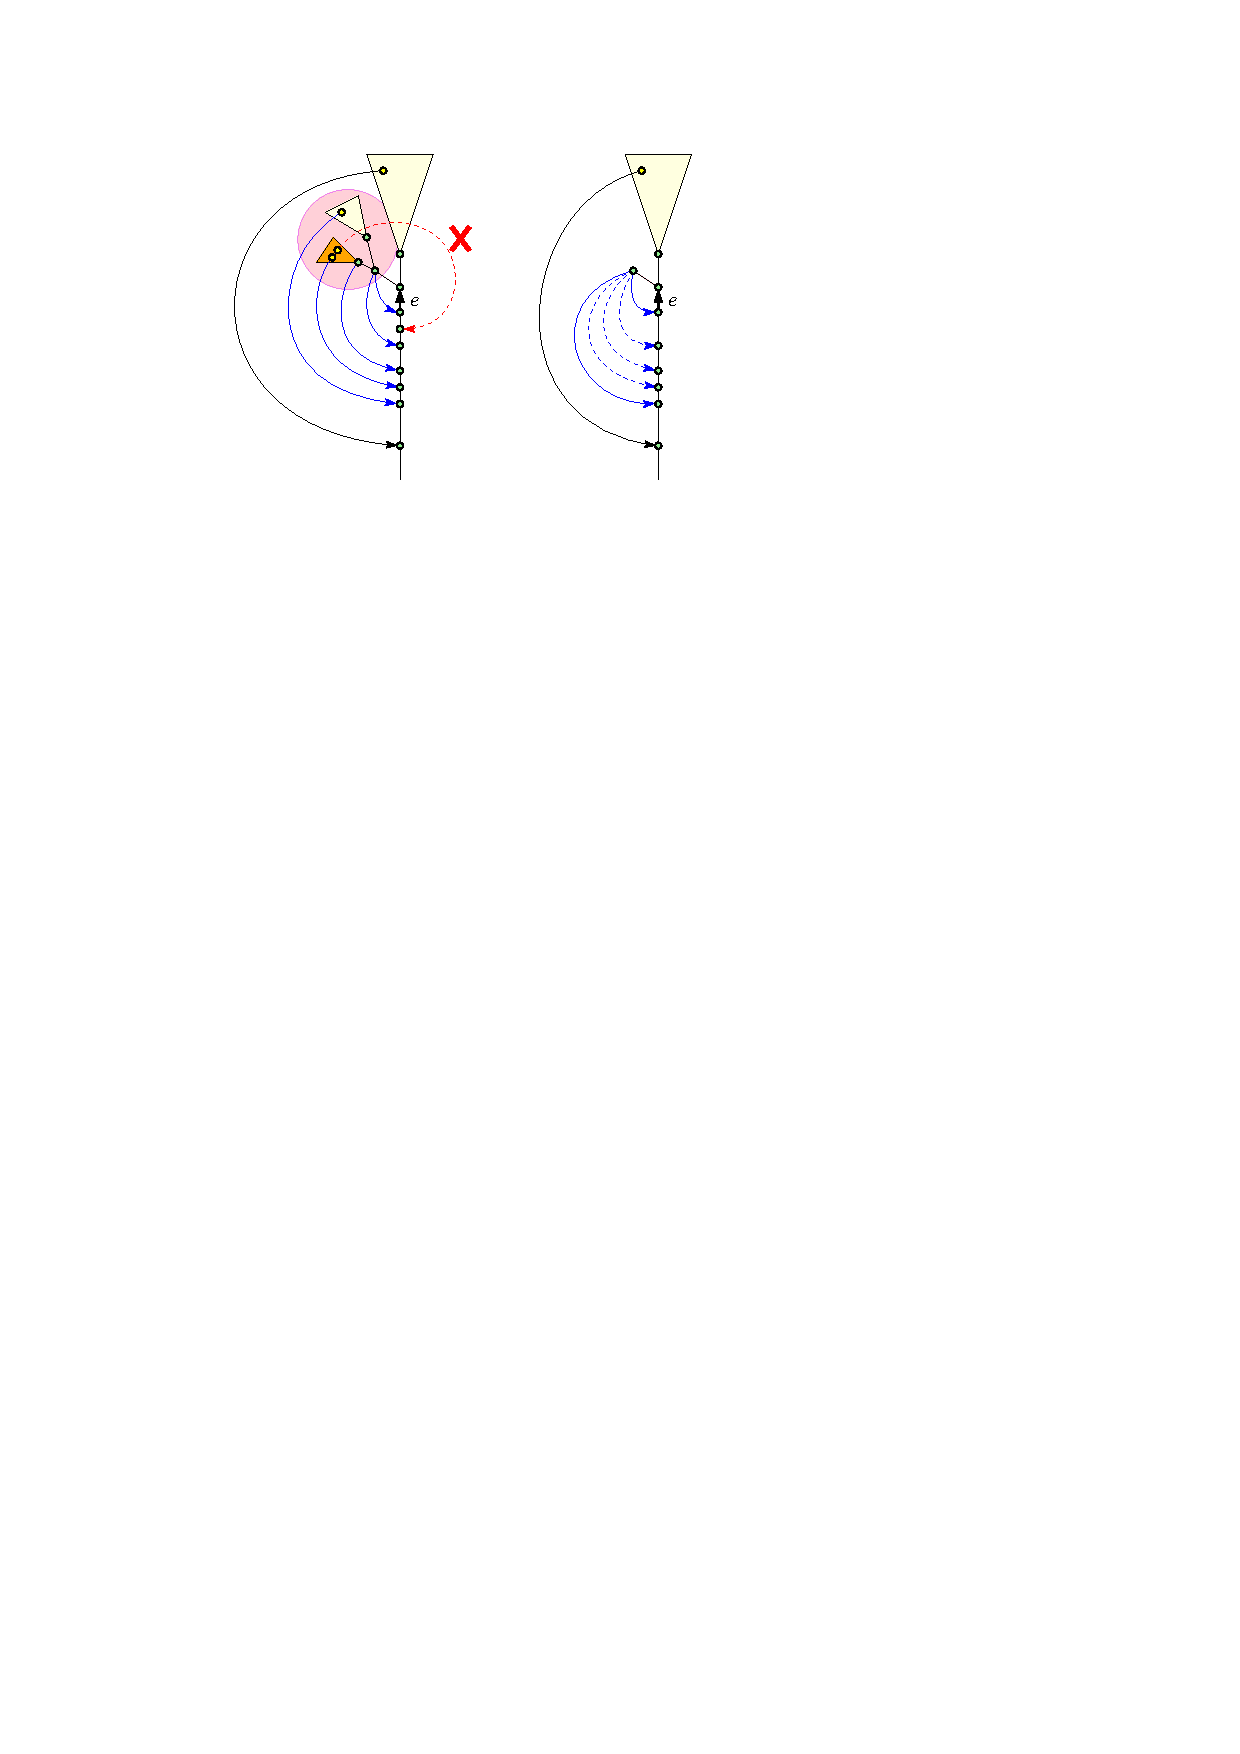
\includegraphics[width=0.31\textwidth]{figures/merge_t_alike_edges.pdf}

\end{paracol}


右図左の丸で囲まれたフリンジを縮約対象とし考察する。右が所望の縮約結果である。
すべての補木辺が{\tt left}サイドに配置されているならクラフトスキーグラフは存在しない。
$\low(e_1)$を終点とする補木辺が存在するので、
いずれの補木辺も部分的に{\tt right}に配置することはできない。
{\tt right}に配置する場合は全ての補木辺を{\tt fops}内の順序を変えること無く
移動させなければならない。
以上のことから
仮想的な頂点を始点とするよう縮約して扱う必要がある。



\begin{lstlisting}[language=Python, caption=\_merge\_t\_alike\_edges,escapechar=@,
                   label=lst:_merge_t_alike_edges]
    def _merge_t_alike_edges(self):
        if self.H.right:
            raise Exception
        for f in islice(self.fops, 1, len(self.fops)):
            if f.right:
                raise Exception
            self.H.left.extend(f.left)
        self.fops = deque([self.fops[0]])
\end{lstlisting}



このときオレンジの部分木のように、
{\tt left, right}両サイドに補木辺が配置されるフリンジ内干渉が存在する場合
クラフトスキーグラフを形成する。
第2行および第5行のように{\tt if self.H.right}で非空を判定し、
真のとき例外{\tt Exception}を生成し平面的でないと判定し処理を完了する。
そうでない場合は第7行のように、
先頭のフリンジ内干渉の双方向キュー{\tt left}の末尾に連結する。
最終的に第8行のように唯一のフリンジ内干渉に縮約されるので、
参照点{\tt H}の利用はそれほど本質的ではない。

\paragraph{計算量と正当性}
\lstrefname\ref{lst:_merge_t_alike_edges}の
第4行の{\tt for}ループの内部は1つの条件式と連結リストの結合なので$O(1)$。
ループ回数はフリンジ内干渉のリスト{\tt fops}のサイズなので
$O(|\omega^+(v)|+|\omega^-(v)|)$で抑えられる。
正当性は\cref{lemma:t_alike}に従う。

\begin{lemma}
\label{lemma:t_alike}
\lstrefname\ref{lst:_merge_t_alike_edges}が例外を生成するなら
クラトフスキー部分グラフが存在する。
\end{lemma}



\setcolumnwidth{0.66\textwidth, 0.33\textwidth}
\begin{paracol}{2}
\begin{proof}
{\tt right}が非空になる二通りの場合を考察する。

まず、フリンジ内干渉を形成するには、右図左下段のように五つの頂点の下で、
三つの補木辺(シアン)と四つの木辺(黒)が少なくとも必要である。
%五頂点のうち補木辺の始点と終点の組合せは右図のように上$2$下$3$以外に
%上$3$下$2$も考えられる。
補木辺の始点の中で最も根に近い頂点を$v$、終点の中で最も根から離れている頂点を$x$とする。
\lstrefname\ref{lst:_merge_t_alike_edges}が呼ばれる状況、つまり
${\mathcal T}_v$の頂点を始点とする補木辺を継承して
フリンジを形成することを考える。
%このとき\cref{lemma:ignoring_back_edges}は、
%$v$を始点とする補木辺か
%$x$を終点とする補木辺%のいずれか
%を対象外とするので、
このとき、木辺$(x, v)$を細分するような頂点$y$が存在し、
$y$を始点とし高さが$h(\low((y, v)))$以下の頂点を終点とする別の
補木辺も存在するとする(右図赤辺)。
頂点と辺の個数$n,~m$を見積もるとそれぞれ$n=6, m=9$を得る。
この部分グラフの内周$\gamma$は$4$なので
\cref{coro:girth}より
平面的グラフなら
$m \leq \frac{\gamma}{\gamma-2}(n-2)$を満たさなければならないが
$9\leq 8$となる。
これは$K_{3,3}$の細分を形成することを意味する。

別の{\tt right}が非空の場合を考察する。
右図の$\omega^-(v)$と$\omega^-(w)$は互いに干渉するので、
{\tt right}が非空のフリンジ内干渉を形成する。
いま木辺$(x, y)$のフリンジを形成しようとしている。
先ほど同様$y$を始点とし高さが$h(\low((y, v)))$以下の頂点を終点とする別の
補木辺も存在するとする(右図赤辺)。
このとき右図右のように黒辺が存在しなければ平面埋込みは存在するが、
黒辺が存在するので平面性は成り立たない。
$\{r, x, y, v, w\}$が導出する部分グラフは$5$-頂点で$4$-正則なので
$K_5$を形成する。

いずれの場合もクラトフスキー部分グラフを形成する。
\end{proof}

%木辺の系列内の中央三つ目の頂点がフリンジを形成しようとしている木辺$(x, y)$の終点$y$にあたる。
%木辺の個数は\cref{coro:ignoring_back_edges}から、
%3つの補木辺は異なる二つの始点と異なる三つの終点が必要な事実に則る。


%根に近い方から三つ目の木辺を細分して分断に使った頂点を$y$、
%$y$の根に近い方の隣接頂点を$x$とする。
%これは\cref{coro:ignoring_back_edges}から、
%$x$の子孫に補木辺の始点となる三つ必要であり、
%同様に$y$の先祖にも任意の補木辺の終点となる三つの異なる頂点が存在しなければならない
%事実に基づく。

%また、アルゴリズムの入力条件として$\low(y)$を終点として持つ補木辺を含む
%別のフリンジが存在する。
%このとき木辺$e=(x, y)$のフリンジを形成することを考える。
%$e_1$として$y$と$\low(e)$を接続する辺が存在する。
%ここまでで頂点は少なくとも$6$、木辺は$5$、補木辺は$4$存在する。

%従って、
%上記$4$つの初等閉路が誘導する部分グラフはクラトフスキー部分グラフを形成する。


\switchcolumn
\vspace{2.\intextsep}
%\centering
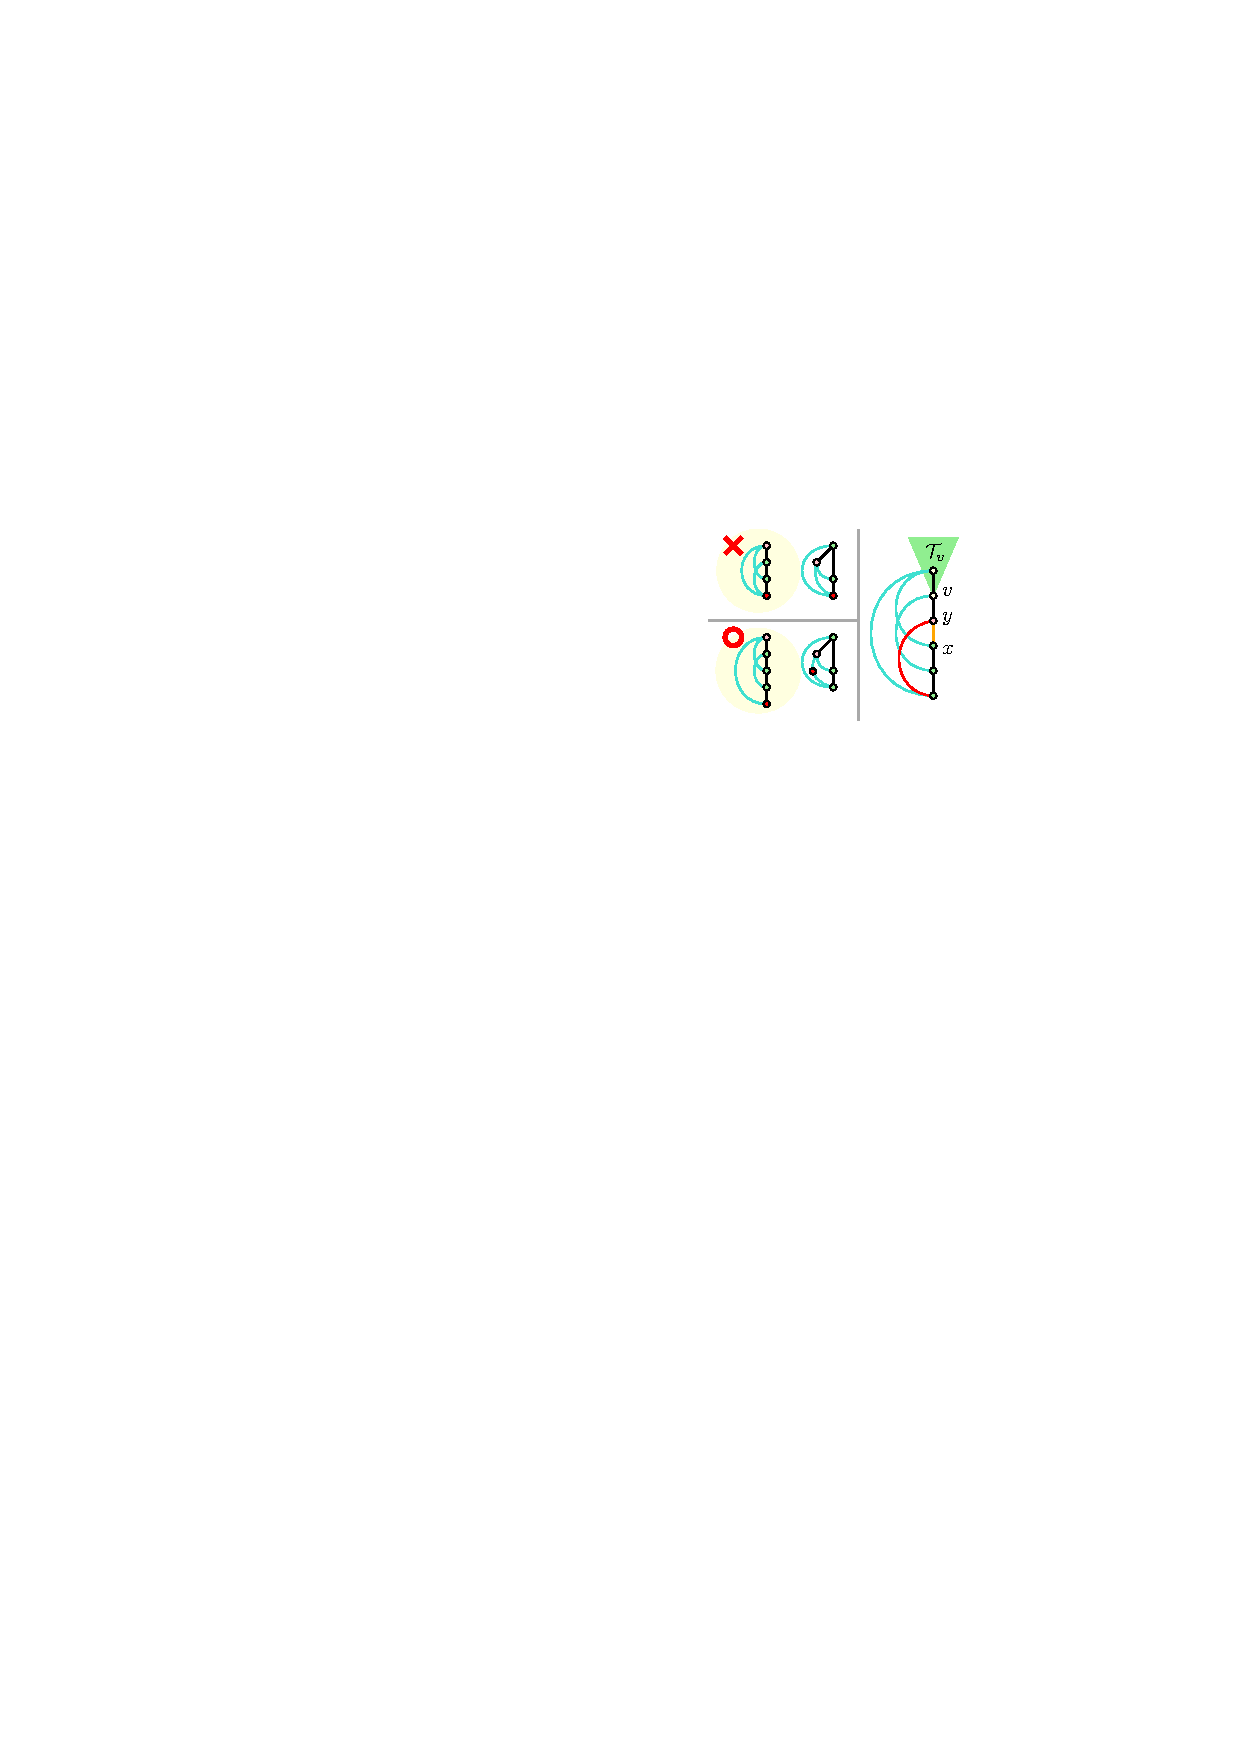
\includegraphics[width=0.29\textwidth]{figures/forbidden_fringe2.pdf}\\
%{\small 左下段は、いずれかの補木辺の内部に根を埋め込まなければならず、
%根は外面に属すという前提に反する。
%従って、内側の補木辺のどちらかは{\tt right}に配置される。}\\
\vspace{0.5\intextsep}
\centering
\includegraphics[width=0.32\textwidth]{figures/proof_onions.pdf}
%\vspace{.5\intextsep}
%\hspace{-1.8em}
%{\small 内周はグラフの最小閉路のサイズであり、閉路が存在しない場合は$\infty$をとる。}
\end{paracol}






\setcolumnwidth{0.6\textwidth, 0.4\textwidth}
\begin{paracol}{2}
\paragraph{正しい玉ねぎ構造の埋込み}
次の禁止グラフの検出は、
対象木辺$e=(x, y)$に対する
$e_1, e_2 \in \omega^+(y)$のフリンジの併合に関する手続きである。
$h(\low(e_1)) \leq h(\low(e_2))$とする。
また$\fringe(e_1)$は{\tt right}が
非空のフリンジ内干渉$\gamma_1=([h(u_2), h(u_1)], [h(u_3)])$を持つ。
ただし、$h(u_1) < h(u_2)$かつ$h(u_1) \leq h(u_3) \leq h(u_2)$。
同様に$\fringe(e_2)$は{\tt right}が空だが$\gamma_1$と干渉する
$\gamma_2=([h(v)], [~])$を持つ。
$\gamma_1$と$\gamma_2$が干渉する場合$h(u_3)$と同様に
$h(u_1) \leq h(v) \leq h(u_2)$を満たす。
このとき$h(v) < h(u_3)$ならクラトフスキー部分グラフを形成する(右図右)。

\switchcolumn
\vspace{1.5\intextsep}
\centering
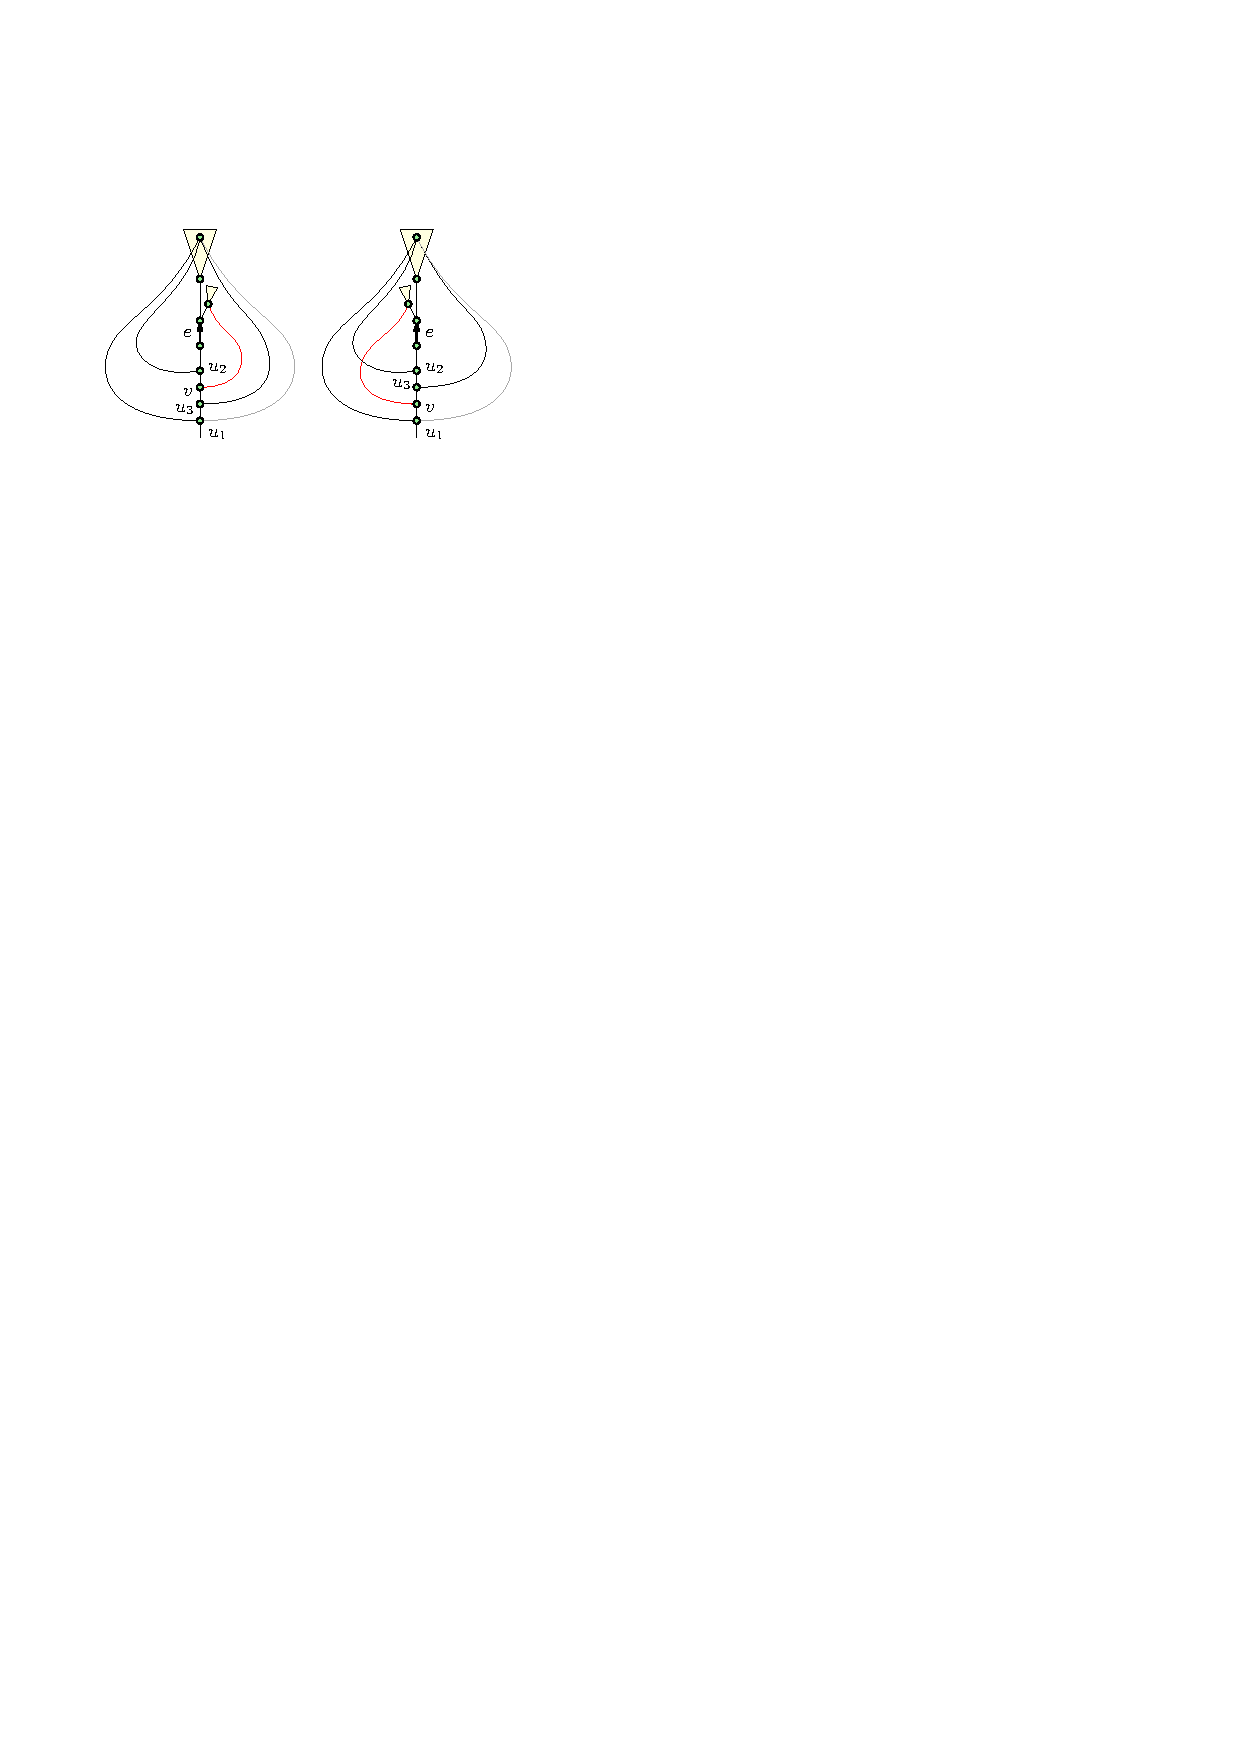
\includegraphics[width=0.37\textwidth]{figures/make_onion.pdf}
\end{paracol}

具体的なpythonコードの例を\lstrefname\ref{lst:_make_onion_structure}に示す。
{\tt self}が$\fringe(e_1)$で{\tt other}が$\fringe(e_2)$。
このとき{\tt self}の
最も根から離れている終点の高さ{\tt self.H.l\_hi}および{\tt self.H.r\_hi}を見て
いずれかの内部に{\tt other}のフリンジ内干渉を埋め込めるかを確認する(第2・3行)。
埋め込めるようであれば{\tt self}の双方向キューに{\tt other}の要素を連結する(第6-9行)。
それ以外の場合は非平面的なので処理を完了する(第4行)。





\setcolumnwidth{0.72\textwidth, 0.28\textwidth}
\begin{paracol}{2}
\begin{lstlisting}[language=Python, caption=\_make\_onion\_structure,
                   label=lst:_make_onion_structure]
    def _make_onion_structure(self, other):
        lo, hi = (0, 1) if self.H.l_hi < self.H.r_hi else (1, 0)
        if other.H.l_lo < self.H.c[lo][0]:
            raise Exception
        elif other.H.l_lo < self.H.c[hi][0]:
            self.H.c[lo].extendleft(reversed(other.H.left))
            self.H.c[hi].extendleft(reversed(other.H.right))
            other.H.left.clear()
            other.H.right.clear()
\end{lstlisting}


\switchcolumn
\vspace{1.\intextsep}
\centering
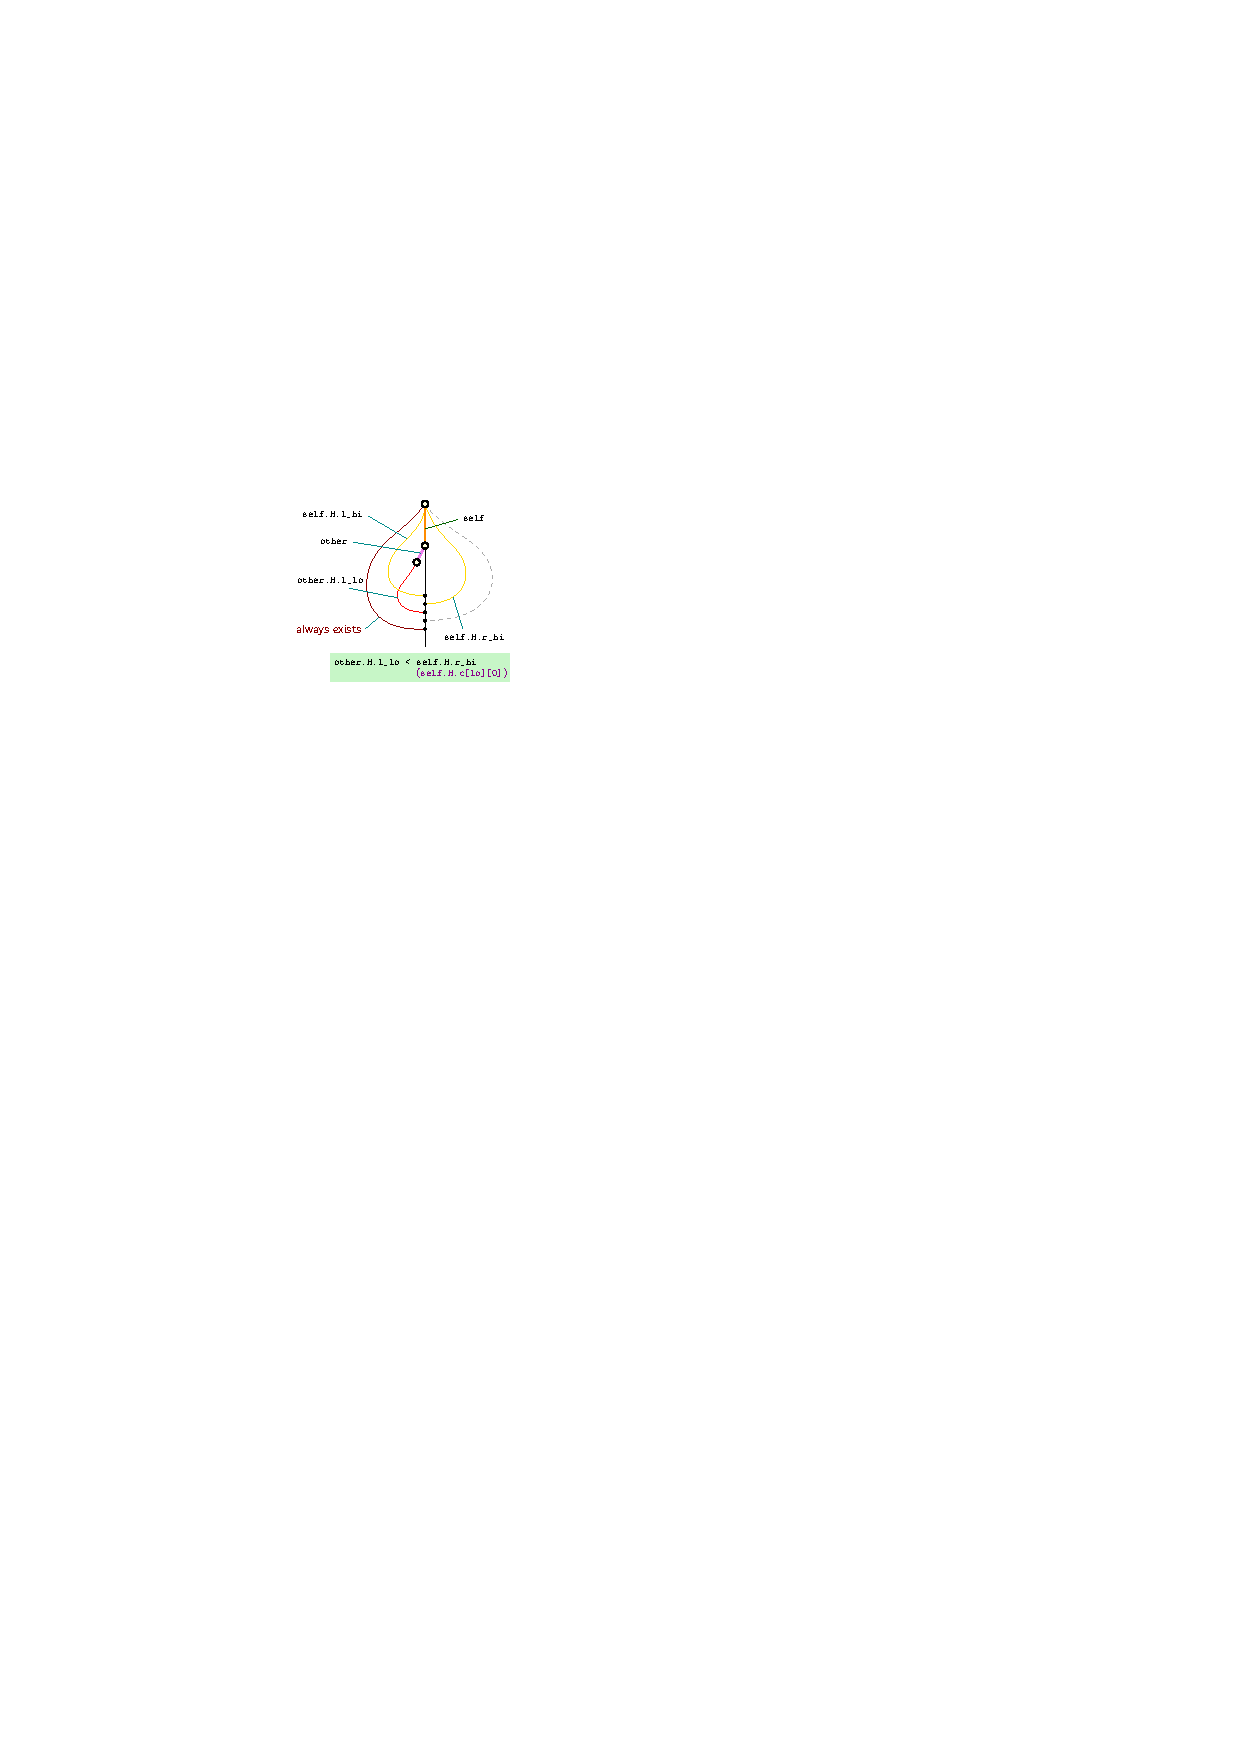
\includegraphics[width=0.27\textwidth]{figures/illegal_onion_conditions.pdf}
\end{paracol}

玉ねぎ構造という名称は別にふざけて呼んでいるわけではない。
幾何学的グラフに準ずる組合せ構造の列挙や数え上げに対して
用いられる層構造を呼称する際に用いられている。
また、平面的グラフを対象とする最適化問題の多くは、
ベイカーのやり方に代表される層構造を利用したアプローチが広く用いられる。

\paragraph{計算量と正当性}
\lstrefname\ref{lst:_make_onion_structure}は
三つの条件式および連結リストの結合と破棄なので$O(1)$で完了する。
pythonの{\tt collections.deque.extendleft}は最悪の場合
$O(|\omega^+(v)|+|\omega^-(v)|)$時間かかるので
必要に応じて実装を見直す必要がある。
ただ、ここで結合された要素は以降のフリンジ形成において削除されるまで
入れ替えられることはないので全体の計算量へは漸近的に影響しない。
また、正当性は\cref{lemma:onion}に従う。

%\setcolumnwidth{0.85\textwidth, 0.15\textwidth}
%\begin{paracol}{2}
\begin{lemma}
\label{lemma:onion}
\lstrefname\ref{lst:_make_onion_structure}が例外を生成するなら
クラトフスキー部分グラフが存在する。
\end{lemma}


\begin{proof}
\cref{lemma:t_alike}の証明と同様の議論が成り立つ。
\cref{lemma:t_alike}では、
{\tt right}が空のフリンジ内干渉に対して
{\tt right}が非空のフリンジ内干渉を併合する手続きだが、
ここではその逆の場合なので結局クラトフスキー部分グラフを持つ。
%
%
%とりうる場合は二通りある。
%前者は、\cref{lemma:t_alike}において
%シアンの補木辺の集まりを{\tt self}、赤の補木辺を{\tt other}と見立てる逆の構成であり、
%後者は右図に示す
%緑の部分木${\mathcal T}_v$の補木辺の集まりを{\tt self}、
%赤辺を{\tt other}とする構成である。
%前者は$K_{3,3}$の細分となり、
%後者は$5$-頂点$4$-正則なグラフなので$K_5$の細分となる。
\end{proof}

%\switchcolumn
%\vspace{0.5\intextsep}
%\centering
%\includegraphics[width=0.1\textwidth]{proof_onions.pdf}
%\end{paracol}




\subsubsection{補木辺の削除}
バックトラックでクラトフスキーグラフを検出しなかった場合、
先祖のフリンジに継承されない補木辺を破棄する手続きを確認する。
すなわち$T_{\succeq y}=\{(u, v) \in E \setminus T ~|~ y \preceq v\}$。
具体的なpythonコードを\lstrefname\ref{lst:prune}に示す。
バックトラックで$\fringe(e)$を形成し終えた直後に、
禁止グラフが存在しなかったら$e$の終点に接続する辺を破棄する。
下図は{\tt left}しか明示していないが{\tt right}も同時に確認していく。
玉ねぎ構造の内側{\tt self.H}から順次破棄する。

\setcolumnwidth{0.85\textwidth, 0.15\textwidth}
\begin{paracol}{2}
\begin{lstlisting}[language=Python, caption=prune,
                   label=lst:prune]
    def prune(self, dfs_height):
        left_, right_ = self.__lr_condition(dfs_height)
        while self.fops and (left_ or right_):
            if left_:
                self.H.left.popleft()
            if right_:
                self.H.right.popleft()
            if not self.H.left and not self.H.right:
                self.fops.popleft()
            else:
                self._swap_side()
            if self.fops:
                left_, right_ = self.__lr_condition(dfs_height)
\end{lstlisting}
\switchcolumn
\vspace{2.5\intextsep}
\centering
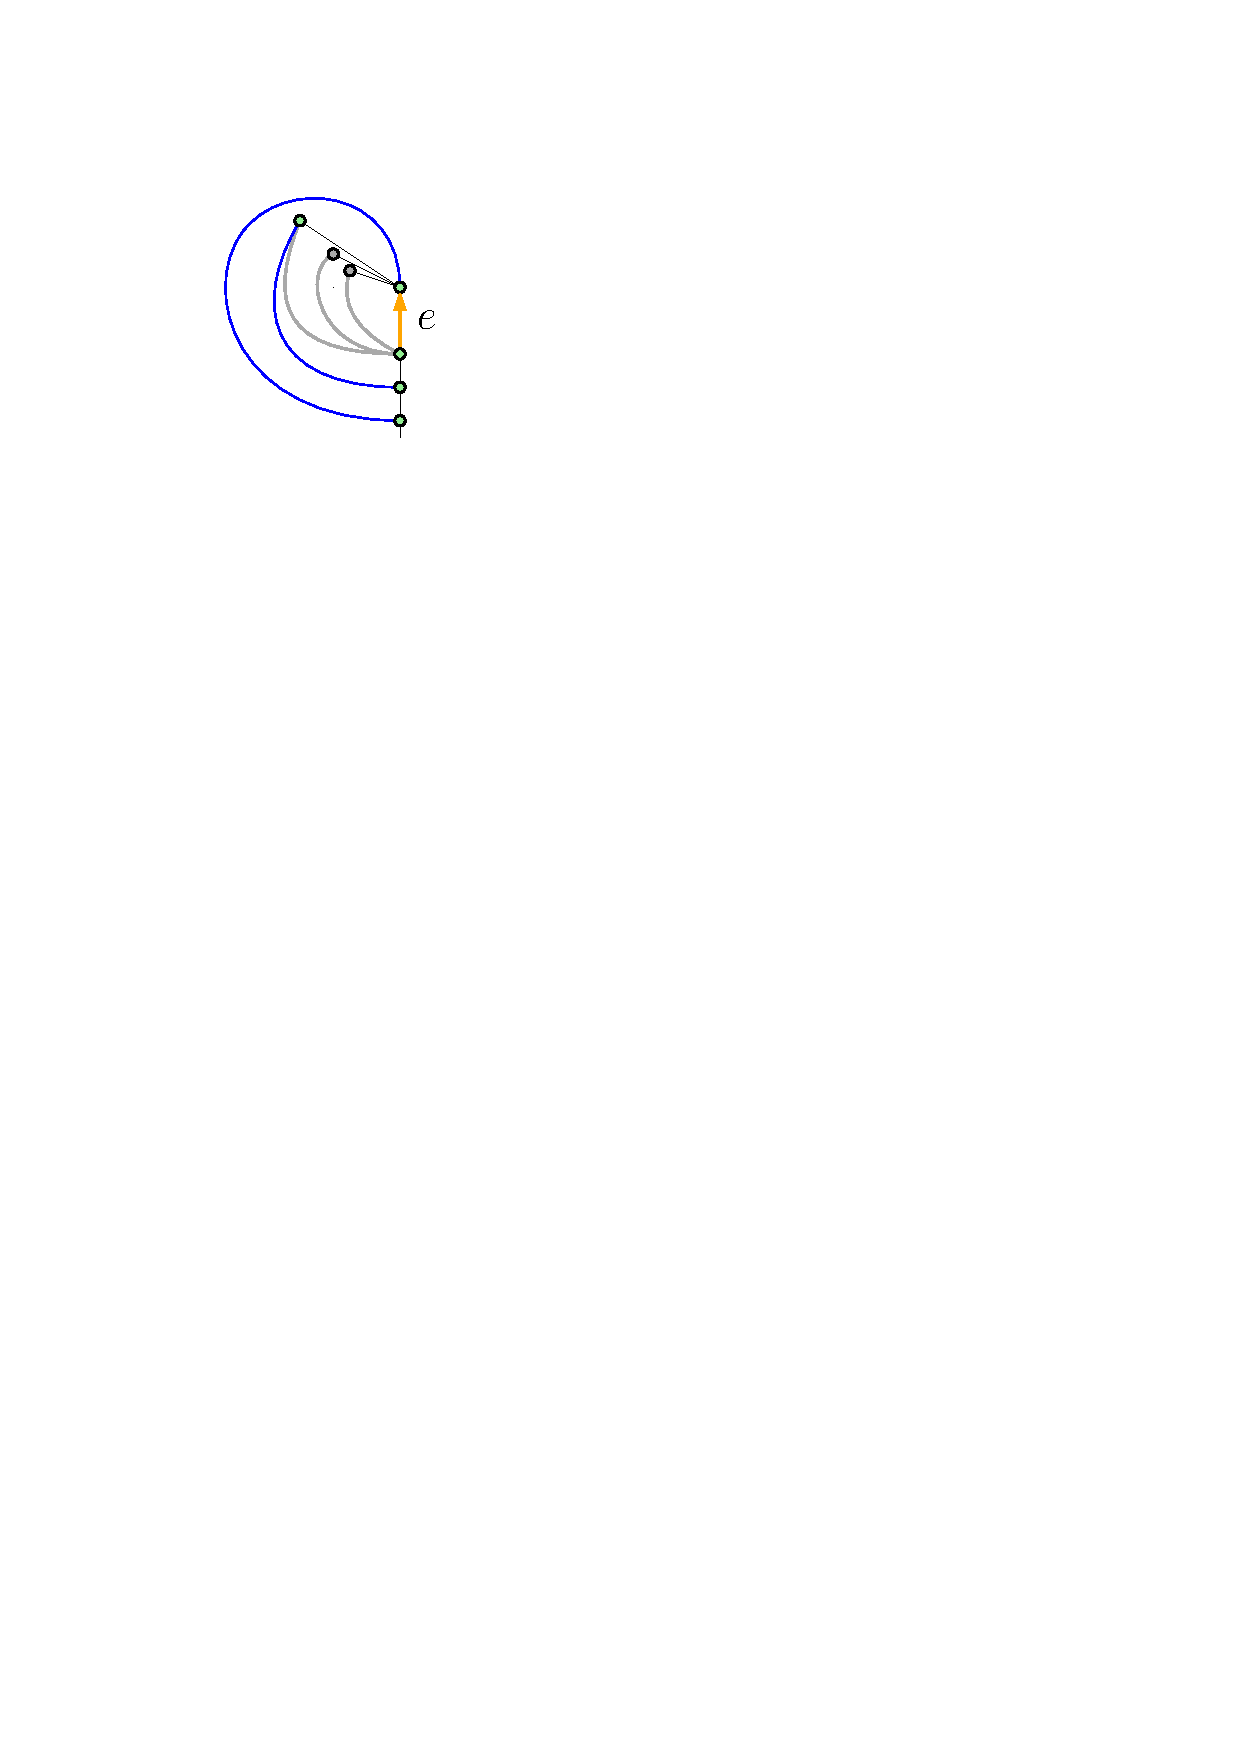
\includegraphics[width=0.14\textwidth]{figures/prune_in_fringe.pdf}
\end{paracol}

\lstrefname\ref{lst:prune}~({\tt prune})は二つの手続き{\tt \_\_lr\_condition}と{\tt \_swap\_side}を呼び出す。
前者は両サイドの双方向キューの存在確認で、後者は管理規約に従い{\tt left}が空で{\tt right}が
非空の場合に置換する手続きである。

\begin{lstlisting}[language=Python, caption=\_\_lr\_condition,
                   label=lst:lr_condition]
    def __lr_condition(self, dfs_height):
        return (self.H.left and self.H.l_hi >= dfs_height,
                self.H.right and self.H.r_hi >= dfs_height)            
\end{lstlisting}


\begin{lstlisting}[language=Python, caption=\_swap\_side,
                   label=lst:swap_side]
    def _swap_side(self):
        if not self.H.left or (self.H.right and self.H.l_lo > self.H.r_lo):
            self.H.c[0], self.H.c[1] = self.H.c[1], self.H.c[0]
\end{lstlisting}



\paragraph{計算量と正当性}
フリンジ内干渉のデータ構造の管理規約により正しく入れ子構造が保証できるので
$O(|\omega^+(v)|)$時間で完了する。
$\omega^-(v)$が勘定に入っていないのは
対象グラフとして単純グラフを想定しているからである。
正当性は\cref{lemma:swap_side}が保証する。

\begin{lemma}
\label{lemma:swap_side}
左優先の管理規約において、
アルゴリズムの処理過程で{\tt left}が空集合で{\tt right}が非空となる場合、
{\tt right}の補木辺集合を{\tt left}に置き換えても写像が交差することはない。
\end{lemma}

\setcolumnwidth{0.66\textwidth, 0.33\textwidth}
\begin{paracol}{2}
\begin{proof}
{\tt left}が空で{\tt right}が非空になる唯一の経緯を演繹的に置換操作が
問題無いことを示す。

木辺$e=(x, y)$のフリンジを形成する状況で、
$e_1=(y, u),~ e_2=(y, v) \in \omega^+(y)$が互いに干渉する場合を考える。
$h(\low(e_1)) < h(\low(e_2))$で、
$\omega^-(u)$が
\lstrefname\ref{lst:_merge_t_alike_edges}に基づき
縮約されているとする。
このとき\lstrefname\ref{lst:t_opposite}に基づき$\fringe(e_1)$を{\tt right}に配置する
フリンジ内干渉が形成される。
禁止グラフを検出しないまま$w=\low(e_2)$までバックトラックし$w$の先祖に進む直前で
$\fringe(e_2)$は禁止グラフを引き起こす可能性のある補木辺は一つもなくなる。
一方で$\low(e_1)$を終点として持つ補木辺は存在する。
この状況で\lstrefname\ref{lst:swap_side}に基づき
フリンジ内干渉の{\tt left}と{\tt right}を置換しても矛盾を誘発しない。
%
\end{proof}
\switchcolumn
\vspace{1.\intextsep}
\centering
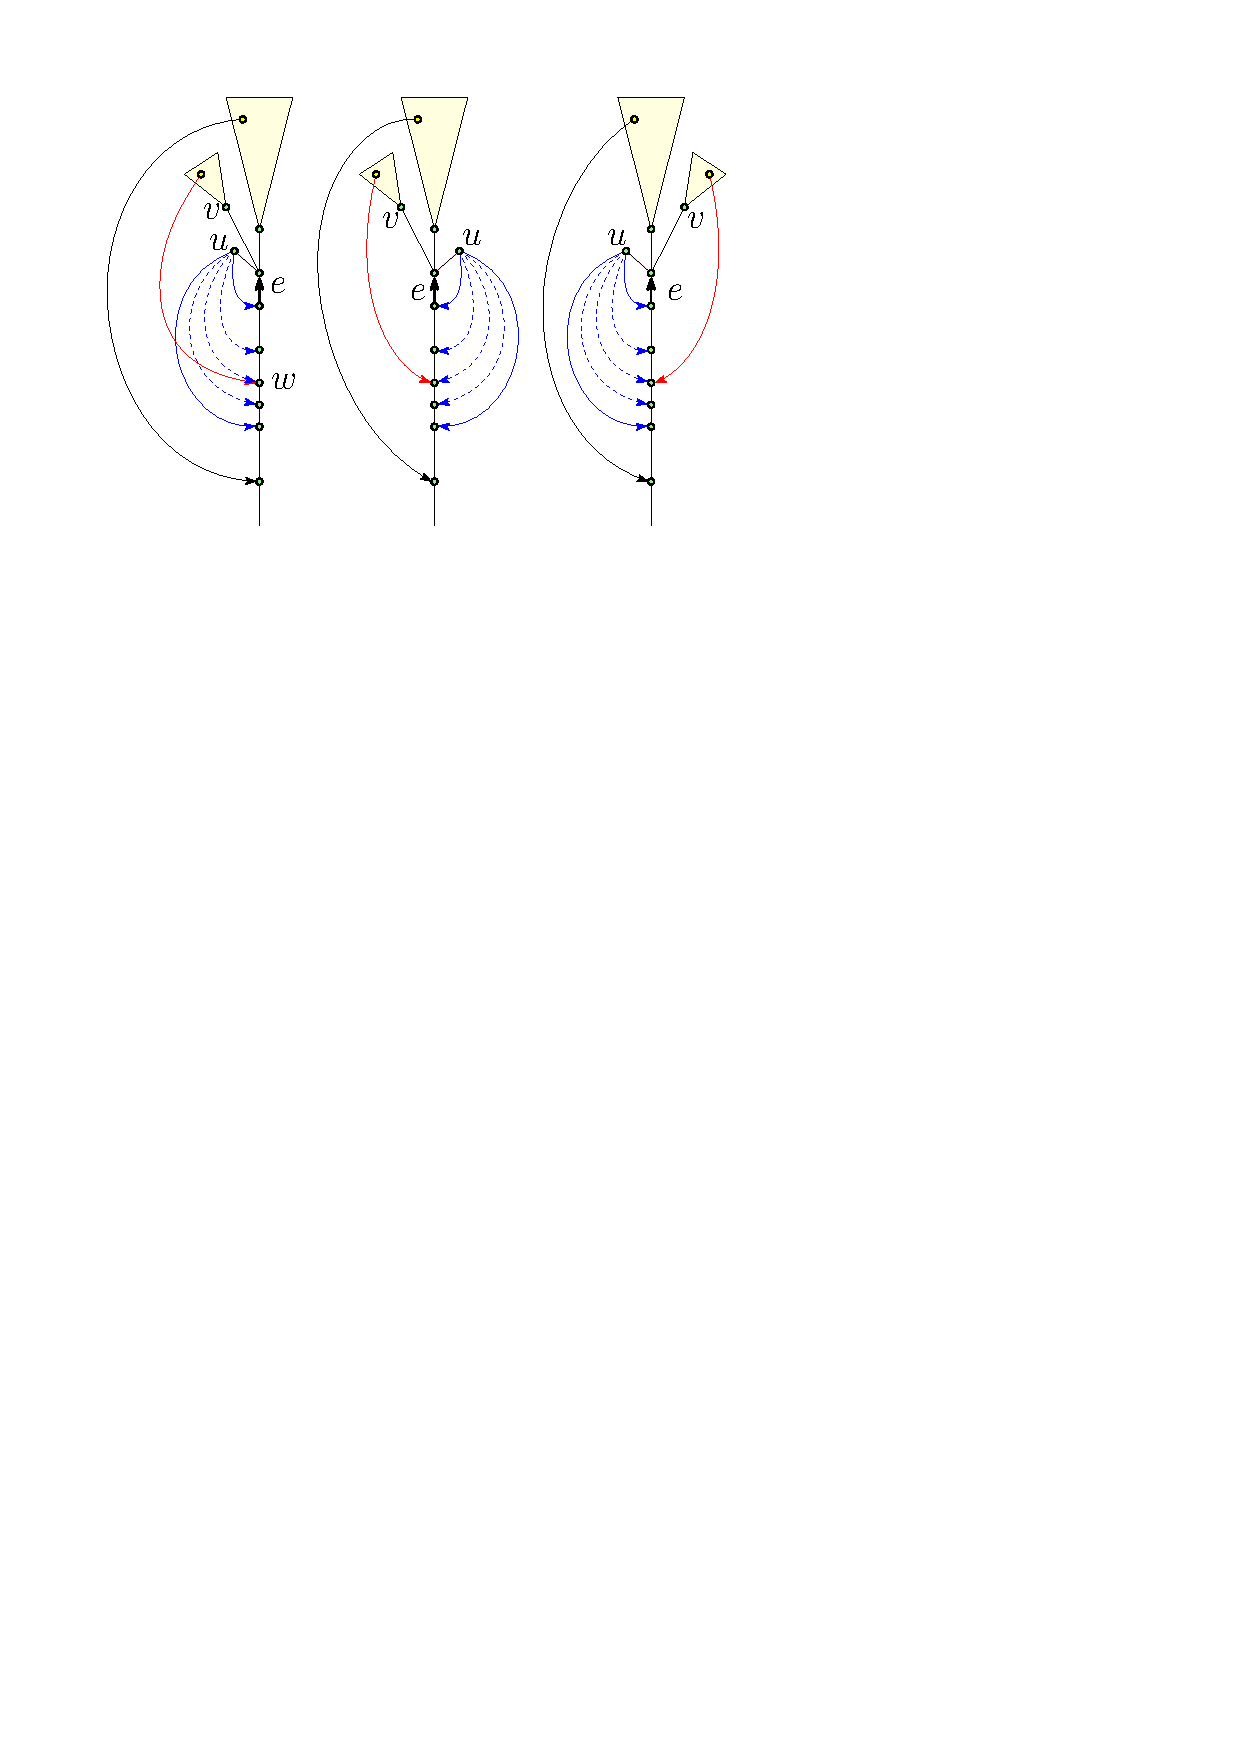
\includegraphics[width=0.32\textwidth]{figures/swap_side.pdf}
\end{paracol}



\subsection{F-彩色による平面性保証}
前節では
\lstrefname\ref{lst:is_planar}~{\tt is\_planar}が
非平面的と答えたら与えられたグラフは非平面的であることを
証拠付きで保証できることを確認した。
残りはアルゴリズムが平面的と答えた場合の正当性を保証しなければならない。
これはF-彩色性という概念を用いる。

\begin{definition}[F-彩色]
グラフ$G = (V, E)$とその深さ優先探索木$\mathcal{T} = (V, T)$の下で
彩色 $\lambda ~:~ E \setminus T \rightarrow \{{\sf left, right}\}$ が
次の条件を満たすときF-彩色という。
\begin{itemize}
\item 各頂点 $v \in V$ およびその任意の木辺対 $e_1, e_2 \in \omega^+(v)$ に関して
    $\fop_{e_1}(e_2)$ と $\fop_{e_2}(e_1)$ がそれぞれ同色で、
    互いに異なる彩色となる。
\item 同様に、任意の木辺 $e \in \omega^+(v)$ と補木辺 $f \in \omega^-(v)$ の対に関して
    $\fop_e(f) \neq \varnothing$ なら 
    $\fop_{f}(e)$ に属す補木辺すべて同色でかつ、
    各 $f' \in \fop_f(e)$ に関して $\lambda(f') \neq \lambda(f)$ となる。
\end{itemize}
また、あるグラフ$G$が{\sf F}-彩色を許容するなら、$G$はF-彩色を持つ、
もしくはF-彩色性を有するという。
\end{definition}

F-彩色は補木辺の集合を二つの互いに素な部分集合に分割する。
{\sf left}に彩色された補木辺は、その初等閉路が左回りになり、
{\sf right}の補木辺は右回りになるような平面描画を与える。



\begin{theorem}[F-彩色定理]
$G=(V, E)$を平面的グラフ、${\mathcal T}$をその深さ優先探索木とする。
このとき$G$はF-彩色を持つ。
\end{theorem}


\setcolumnwidth{0.75\textwidth, 0.25\textwidth}
\begin{paracol}{2}
\begin{proof}
$G$は根が外面になるように平面に埋め込まれていると仮定する。
関数$\lambda$を与えられた補木辺に対し、
その初等閉路が左回りなら$\lambda(e)=1$、
右回りなら$\lambda(e)=-1$を返す関数とする。

$v\in V$および$e_1, e_2 \in \omega^+(v)$とする。
$g_1=\fargmin_{(x', y') \in \fringe(e_1)} h(y')$とし
$g_2$も$e_2$に関して同様に定義する。
$\gamma$を次の四つの便宜上無向辺とみなす
辺の系列をつなげた閉路とする。
$g_1$から$g_1, g_2$の終点間の木辺の系列へ、
それから$g_2$に続いて$g_1, g_2$の$v$を経由する木辺の系列(右図緑閉路)。
$u=\argmax_{e\in\{e_1, e_2\}}h(\low(e))$とする。
$C_1,~ C_2$をそれぞれ$g_1, g_2$の初等閉路に対応する写像円とする。
同様に$C_\gamma$を$\gamma$の写像円とする。
$\gamma_1, \gamma_2$をそれぞれ$g_1, g_2$の写像円とする。
$P$を$u$から$v$への木辺の系列とする。
このとき互いに独立な二つの場合を考える。

$P$が$C_\gamma$の内部にある(右図上)。
このとき
例えば$\lambda(g_1)=1,~ \lambda(g_2)=-1$のように
$g_1$と$g_2$は異なる彩色がなされ、
$P$の左に$C_1$、右に$C_2$ガ描画される。
$\fop_{e_2}(e_1)$のどの補木辺の写像も$\gamma_1$と交差しないし
同様に$\fop_{e_1}(e_2)$のどれも$\gamma_2$と交差しないので、
$\lambda(f_1)=\lambda(g_1)$および$\lambda(f_2)=\lambda(g_2)$を得る。

$P$が$C_\gamma$の外部にある(右図下)。
$g_1$と$g_2$は同色の彩色がなされ、$C_1$が$C_2$を包含する。
このとき$P$の左は$C_1$に属し、右は$C_2$外部に属す。
$\fop_{e_2}(e_1)$のどの補木辺も$\gamma_2$と交差しないし
同様に$\fop_{e_1}(e_2)$のどの辺の写像も$\gamma_1$と交差しない。
従って$\lambda(f_1)=-\lambda(g_1)$および$\lambda(f_2)=\lambda(g_2)$を得る。


いずれの場合も$\fop_{e_2}(e_1)$と$\fop_{e_1}(e_2)$はそれぞれ同一色で、
互いに異なる彩色がなされる。従って$\lambda$は$F$-彩色である。
\end{proof}
\switchcolumn
\vspace{.5\intextsep}
\centering
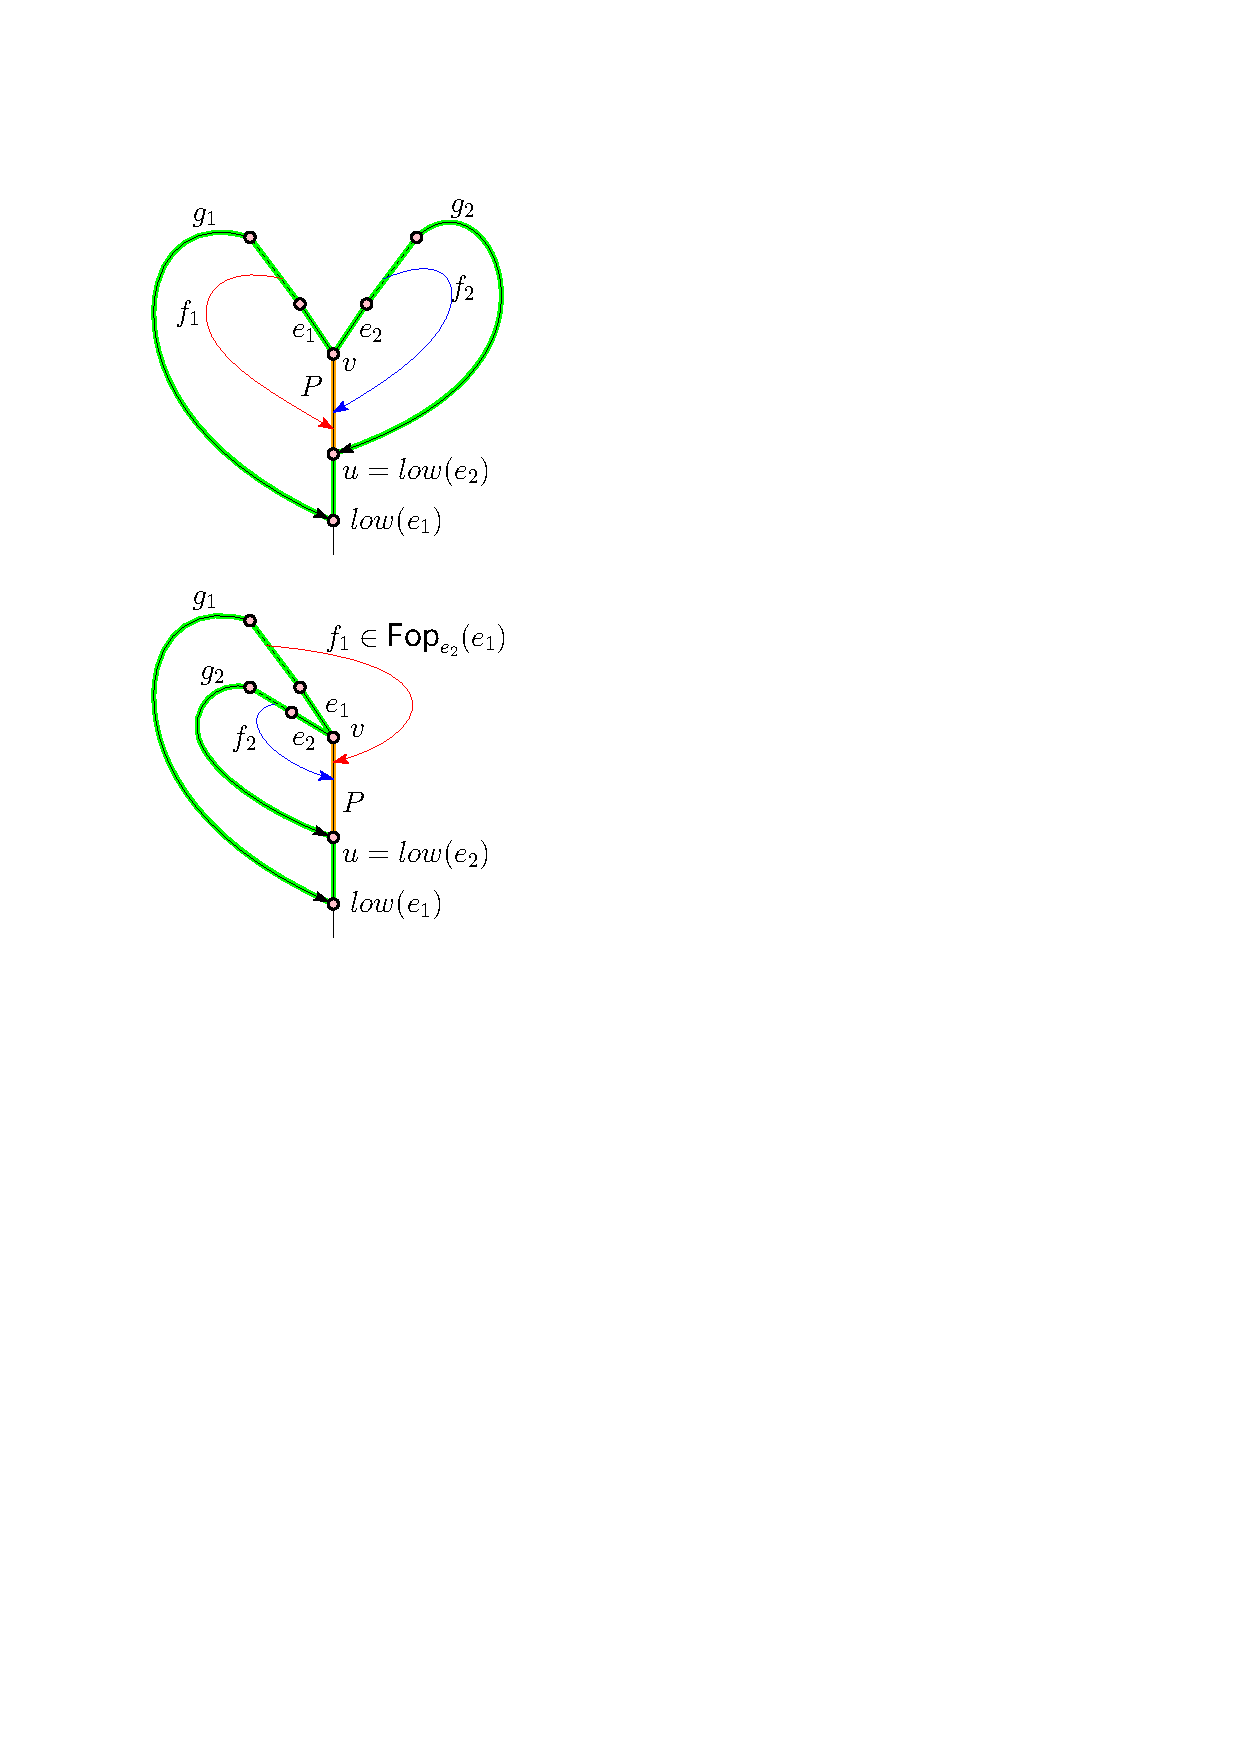
\includegraphics[width=0.23\textwidth]{figures/f_coloring.pdf}
\end{paracol}



\paragraph{F-彩色定理に基づく正当性保証}
最終的に禁止グラフであるクラトフスキー部分グラフを検出しなかったとき
F-彩色が存在することが示せれば、\
\lstrefname\ref{lst:is_planar}({\tt is\_planar})は
正しく平面性を判定することが示せる。

\begin{lemma}
\lstrefname\ref{lst:is_planar}~({\tt is\_planar})で禁止グラフを検出しない場合、
F-彩色が存在する。
\end{lemma}

\begin{proof}
\lstrefname\ref{lst:prune}~({\tt prune})において補木辺が削除されるタイミングで
{\tt left}と{\tt right}いずれに属すかに応じて彩色することを考える。
ただ{\tt left}が空で{\tt right}が非空になると
\lstrefname\ref{lst:swap_side}~({\tt \_swap\_side})による置換が発生することに注意する。
%補木辺が比較対象外となった時点での{\tt left}/{\tt right}に応じて彩色するのではなく、
%例えば

干渉する辺と反対の色が割り当てられるよう記憶しておく。
同様に\lstrefname\ref{lst:_merge_t_alike_edges}
({\tt \_merge\_t\_alike\_edges})の縮約により同色になるべき
先祖に接続する補木辺が存在する場合も適宜記憶する。
従属する補木辺がない場合は、左優先の管理規約に基づき{\sf left}で彩色すれば良い。
この従属関係は対象グラフが平面性を有するなら
閉路のない有向グラフとなるので、
最終的に確定している彩色値に応じて先祖から子孫へ適宜伝搬していけば、
$O(E\setminus T)$時間でF-彩色を得る。
\end{proof}

最終的に次の定理を得る。

\begin{theorem}
\lstrefname\ref{lst:is_planar}~{\tt is\_planar}は
連結なグラフの平面性判定を線形時間で与える。
\end{theorem}


\subsection{クラス{\tt fringe}のpythonコード}
クラス{\tt fringe}の全体を\lstrefname\ref{fringe}に示す。
また、これまで記述した平面性判定に関するpythonコードは
\url{https://github.com/satemochi/is_planar}で管理している。
%すでに{\tt \_merge\_t\_alike\_edges}、{\tt \_make\_onion\_structure}および
%{\tt prune}については詳細を確認したが、
%残りのクラスメソッドについては基本的に
%第\ref{fop_specification}節のフリンジ内干渉のデータ構造に対する管理規約に
%従うよう仕様に則った記述なので解説は割愛する。

\begin{lstlisting}[language=Python, caption=クラス fringe,
                   label=fringe]
class fringe:
    def __init__(self, dfs_h=None):
        self.fops = deque() if dfs_h is None else deque([fop(dfs_h)])

    def __lt__(self, other):
        diff = self.L.l_lo - other.L.l_lo
        if diff != 0:
            return diff < 0
        return self.H.l_hi < other.H.l_hi

    @property
    def H(self):
        return self.fops[0]

    @property
    def L(self):
        return self.fops[-1]

    def merge(self, other):
        other._merge_t_alike_edges()
        self._merge_t_opposite_edges_into(other)
        if not self.H.right:
            other._align_duplicates(self.L.l_hi)
        else:
            self._make_onion_structure(other)
        if other.H.left:
            self.fops.appendleft(other.H)

    def _merge_t_alike_edges(self):
        if self.H.right:
            raise Exception
        for f in islice(self.fops, 1, len(self.fops)):
            if f.right:
                raise Exception
            self.H.left.extend(f.left)
        self.fops = deque([self.fops[0]])

    def _merge_t_opposite_edges_into(self, other):
        while (not self.H.right and self.H.l_hi > other.H.l_lo):
            other.H.right.extend(self.H.left)
            self.fops.popleft()

    def _align_duplicates(self, dfs_h):
        if self.H.l_lo == dfs_h:
            self.H.left.pop()
            self._swap_side()

    def _swap_side(self):
        if not self.H.left or (self.H.right and self.H.l_lo > self.H.r_lo):
            self.H.c[0], self.H.c[1] = self.H.c[1], self.H.c[0]

    def _make_onion_structure(self, other):
        lo, hi = (0, 1) if self.H.l_hi < self.H.r_hi else (1, 0)
        if other.H.l_lo < self.H.c[lo][0]:
            raise Exception
        elif other.H.l_lo < self.H.c[hi][0]:
            self.H.c[lo].extendleft(reversed(other.H.left))
            self.H.c[hi].extendleft(reversed(other.H.right))
            other.H.left.clear()
            other.H.right.clear()

    def prune(self, dfs_height):
        left_, right_ = self.__lr_condition(dfs_height)
        while self.fops and (left_ or right_):
            if left_:
                self.H.left.popleft()
            if right_:
                self.H.right.popleft()
            if not self.H.left and not self.H.right:
                self.fops.popleft()
            else:
                self._swap_side()
            if self.fops:
                left_, right_ = self.__lr_condition(dfs_height)

    def __lr_condition(self, dfs_height):
        return (self.H.left and self.H.l_hi >= dfs_height,
                self.H.right and self.H.r_hi >= dfs_height)                   
\end{lstlisting}


